\documentclass{article}

\newcommand{\dznopagestyle}{}

%; Packages
\usepackage{dztex}
\usepackage{mathtools}
\usepackage{IEEEtrantools}
\usepackage{blkarray}
\usepackage{bigints}
\usepackage{tikz}
\usepackage{setspace}
\usepackage{titling}
\usepackage{ifthen}
\usetikzlibrary{arrows.meta,arrows,positioning}

\usepackage{pgfplots}
\pgfplotsset{compat=1.5.1}
\pgfplotsset{every tick label/.append style={font=\footnotesize}}
%:

%; Commands
\renewcommand{\familydefault}{\sfdefault}
\DeclareMathOperator{\diam}{diam}
\DeclareMathOperator{\hm}{\mathcal{H}}
\DeclareMathOperator{\betop}{\mathcal{B}}
\DeclareMathOperator{\gamop}{\Gamma}
\newcommand{\bet}[1]{\betop\parens{#1}}
\newcommand{\gam}[1]{\gamop\parens{#1}}
\newcommand{\aeven}{\mathcal{A}_{\mathrm{even}}^+}
\newcommand{\aodd}{\mathcal{A}_{\mathrm{odd}}^+}
\newcommand{\bec}[1]{\mathbf{#1}}
\newcommand{\ud}{\mathrm{d}}
\newcommand{\eqlbl}[1]{\opstack{=}{#1}}
\newcommand{\opstack}[2]{\stackrel{\mathclap{\normalfont\tiny \mbox{#2}}}{#1}}
\newcommand{\dby}[1]{\frac{\ud}{\ud #1}}
\newcommand{\sproj}{\mathcal{P}_S}
\newcommand{\lsp}[1]{\mathrm{lsp}\braces{#1}}
\newcommand{\utp}{\mathcal{U}_2^\perp}

\newcommand{\haus}[2]{\mathcal{H}^{#1}\parens{#2}}
\newcommand{\R}[1]{\mathbb{R}^{#1}}
\newcommand{\optparens}[1]{\ifthenelse{\equal{#1}{}}{}{\parens{#1}}}
\newcommand{\U}[1]{\mathcal{U}\optparens{#1}}
\newcommand{\UTP}[1]{\mathcal{U}_2^\perp\optparens{#1}}
\newcommand{\chit}[2]{\overline{\chi}_{#1}\optparens{#2}}
\newcommand{\D}[1]{\mathcal{D}\optparens{#1}}
\newcommand{\A}{\mathcal{A}^{+}}
\newcommand{\Ae}{\A_{\textup{Even}}}
\newcommand{\Ao}{\A_{\textup{Odd}}}
\newcommand{\C}{\mathcal{C}}
\newcommand{\ks}{\kappa_\sigma}
\newcommand{\B}[1]{B\parens{#1}}
\newcommand{\G}[1]{\Gamma\parens{#1}}
\newcommand{\sgn}[1]{\mathrm{sgn}\parens{#1}}
\newcommand{\J}[1]{\mathcal{J}{#1}}
\newcommand{\JJ}[1]{\overline{\mathcal{J}}{#1}}
\newcommand{\Pu}{\mathcal{P}}
\newcommand{\Nu}{\mathcal{N}}


% Hijack \dot
\let\olddot\dot
\renewcommand{\dot}[2]{{#1}\cdot{#2}}
\newcommand{\pdot}[2]{\parens{\dot{#1}{#2}}}
%:

\begin{document}

%; Title, Abstract, TOC
\title{\Huge Non-local Curvature of Curves}
\author{Dan Zimmerman, Brian Seguin}
\date{}
\setlength{\droptitle}{-6em}
\maketitle

\begin{abstract}
  Here we study the non-local curvature of a curve and show that there's a natural asymptotic convergence to classical curvature. Concretely, we first study the asymptotics of circles with arbitrary radii, show that, with the right normalization constant, there's an asymptotic relationship to the inverse of the radius, i.e. the classical curvature of a circle. Next we show that the non-curvature of an arbitrary curve can be approximated by the nonlocal curvature of a circle. Finally we show that arbitrary curves' non-local curvature converge to the curve's classical curvature under the right conditions.
\end{abstract}

\doublespacing
\tableofcontents
\singlespacing

%:

\section{Introduction}%;
\subsection{Background}
Continuing from \cite{seguin:2020}, we aim to determine the appropriate conditions needed to recover classical curvature $\kappa$ from non-local curvature $\kappa_\sigma$ as $\sigma \to 1$. Concretely, this means, for a given curve $\mathcal{C}$ in $n$ dimensions we want to analyze
\begin{equation}
  \kappa_\sigma(z) := \parens{\int_{\aeven} - \int_{\aodd}} \frac{\pdot{a}{t(z)} b - \pdot{b}{t(z)}a}{r^{1+\sigma}} \, d\mathcal{H}^{2n-2}\parens{a, b, r}, \label{def:non-local-curv}
\end{equation}
where $t(z)$ is the unit tangent of $\mathcal{C}$ at $z$, and understand the asymptotics as $\sigma \to 1$.
\subsection{Notation}
In the following, we always use:
\begin{itemize}
  \item $n$ to denote the dimension of Euclidean space $\R{n}$ with $n \ge 1$
  \item $\C$ a curve; contextually this will either be a unit circle or arbitrary
  \item $\lambda : \R{1} \to \R{n}$ the parameterization of a curve $\mathcal{C}$
  \item $\kappa(z)$ the classical curvature of $\mathcal{C}$ at $z \in \mathcal{C}$; $\kappa := \kappa_{\mathcal{C}}(0)$
  \item $\ks(z)$ the non-local curvature \eqref{def:non-local-curv} of $\mathcal{C}$ at $z \in \mathcal{C}$; $\ks := \ks(0)$
  \item $\gamma_{p;v} : \mathbb{R} \to \mathcal{M}$ for any manifold $\mathcal{M}$ is a flow such that $\gamma_{p;v}(0) = p, \, \gamma_{p;v}'(0) = v$
  \item $\omega_{k-1} := \frac{2\pi^{k/2}}{\Gamma\parens{k/2}}$ is the surface area of an $k-1$ dimensional unit sphere embedded in $k$ dimensional space
  \item $\haus{k}{\cdot}$ the $k$ dimensional Hausdorff measure
  \item $\U{E} := \braces{ a \in E \mid \abs{a} = 1 }$; $\U{} := \U{\R{n}}$
  \item $\UTP{E} := \braces{ (a, b) \in \U{E} \times \U{E} \mid \dot{a}{b} = 0 }$; $\UTP{} := \UTP{\R{n}}$
  \item $E^c := \braces{ x \in \R{n} : x \not\in E }$
  \item $E^\perp := \braces{ x \in \R{n} \mid \forall y \in E \, \dot{x}{y} = 0 }$
  \item $\chi_E(x) := \begin{cases} 1 : x \in E \\ 0 : x \not\in E \end{cases}$
  \item $\chit{E}{} := \chi_E - \chi_{E^c}$
  \item $\D{p, u, r} := \braces{ p + \xi v \mid \parens{u, v} \in \UTP{}, \xi \in [0, r) }$
  \item $\A\parens{z} := \braces{\parens{a, b, r} \in \UTP{} \mid \pdot{b}{t(z)} > 0}$; $\A = \A\parens{0}$
  \item $\Ae \parens{z} := \braces{\parens{a, b, r} \in \A{}\parens{z} \mid \haus{0}{\D{z + ra, b, r} \cap \C} \text{ is even}}$; $\Ae := \Ae\parens{0}$
  \item $\Ao \parens{z} := \braces{\parens{a, b, r} \in \A{}\parens{z} \mid \haus{0}{\D{z + ra, b, r} \cap \C} \text{ is odd}}$; $\Ao := \Ao\parens{0}$
  \item $(t, n) := (t(z), n(z))$ are the unit (tangent, normal) vectors of $\C$ at $z$
  \item $v^\perp = \parens{\pdot{v}{t}t + \pdot{v}{n}n}^\perp := \pdot{v}{n} t - \pdot{v}{t} n$ for any $v \in \R{2}$; i.e. a clockwise rotation
  \item $\G{z} := \int_0^\infty e^{-t} t^{z-1} \, dt$
  \item $\B{z_1, z_2} := \int_0^1 t^{z_1 -1} \parens{1-t}^{z_2-1} \, dt = 2\int_0^{\pi / 2} \parens{\sin \theta}^{2z_1 - 1} \parens{\cos \theta}^{2z_2 - 1} \, d\theta = \frac{\G{z_1}\G{z_2}}{\G{z_1+z_2}}$
  \item $\sgn{x} := \frac{x}{\abs{x}}$
  \item $\JJ{f} := \sqrt{\nabla f^T \nabla f}$ for change of variables
  \item $\J{f} := \sqrt{\nabla f \nabla f^T}$ for applying the co-area formula
\end{itemize}
%:

\newpage
\section{Non-local Curvature of Circle in 2D}%;
\begin{theorem}
For a circle of radius $R$ in $\R{2}$
$$
  \ks(z) = \frac{2\sqrt{2}}{\sigma R^\sigma} \B{\frac{1}{2}, \frac{1-\sigma}{2}} n(z)
$$
\end{theorem}
\begin{proof}%;
  To begin, notice $\ks(z) = \ks(0) = \ks$ by symmetry and that
  $$
  \dot{\ks}{t} = \parens{\int_{\Ae} - \int_{\Ao}} \frac{\pdot{a}{t}\pdot{b}{t} - \pdot{b}{t}\pdot{a}{t}}{r^{1+\sigma}} \, d\haus{2}{a,b,r} = 0,
  $$
  thus we only need to worry about $\dot{\ks}{n}$; i.e. we wish to compute
  $$
  \dot{\ks}{n} = \int_{\A} \chit{\Ae}{a, b, r} \frac{\pdot{a}{t}\pdot{b}{t} - \pdot{b}{t}\pdot{a}{t}}{r^{1+\sigma}} \, d\haus{2}{a,b,r},
  $$
  where $\A = \Ae \cup \Ao$. The picture below shows the geometric relationship between a given $a, b, r$ with $t, n$ and $u := 2ra$:

%;
\begin{center}
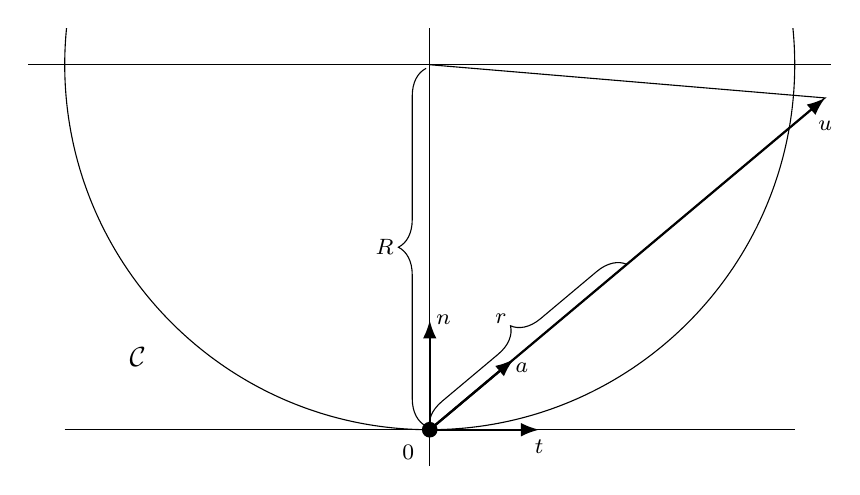
\begin{tikzpicture}
\begin{axis}[ 
    axis lines = middle,
    ticks = none,
    axis line style={-},
    ymin=-1.1, ymax=0.1,
    xmin=-1.1, xmax=1.1,
    axis equal image,
    height=4in
]

%\draw[color=white, fill = blue, opacity=0.2] (axis cs:-1.1, -1) rectangle (axis cs:1.1, 1.1);
%\draw[color=white, fill = gray, opacity=0.4] (axis cs:-1.1, -1.3) rectangle (axis cs:1.1, -1);

\def\figphi{10}
%p/4-phi/2=theta where phi is angle from x-axis of unit circle to top right point of triangle
\def\figtheta{45-\figphi/2}

\draw[color=black] (axis cs:-1, -1) -- (axis cs:1, -1);
  \node at (axis cs:-0.8, -0.8) {$\C$};
%\addplot[data cs=polar, red, opacity=0.6, domain=0:180,samples=180,smooth, fill=red, fill opacity=0.6, shift={(0, transformdirectiony(-1))}] (x, {cos(90 - x)});
\begin{scope}[shift={(0, transformdirectiony(-1))}]
  \node[label={225:{\footnotesize $0$}},circle,fill,inner sep=2pt] at (axis cs:0,0) {};
  %\draw (axis cs:0.25,0) arc(0:{\figtheta}:{transformdirectionx(0.25)});
  %\node at (axis cs:{0.17*cos(0.5*\figtheta)}, {0.17*sin(0.5*\figtheta)}) {$\theta$};
  \draw (axis cs:0,0) -- (axis cs:{1.1*2*sin(\figtheta)*cos(\figtheta)},{1.1*2*sin(\figtheta)*sin(\figtheta)}) -- (axis cs:0, 1);
  \draw [decorate,decoration={brace,amplitude=10pt}] (axis cs:0,0) -- (axis cs:{(1.1/2)*2*sin(\figtheta)*cos(\figtheta)},{(1.1/2)*2*sin(\figtheta)*sin(\figtheta)}) node [black,midway,yshift={transformdirectiony(0.1)}, xshift={transformdirectionx(-0.1)}] {\footnotesize $r$};
  %\draw [decorate,decoration={brace,amplitude=15pt, mirror}] (axis cs:0,0) -- (axis cs:{(1.1)*2*sin(\figtheta)*cos(\figtheta)},{(1.1)*2*sin(\figtheta)*sin(\figtheta)}) node [black,midway,yshift={transformdirectiony(-0.15)}, xshift={transformdirectionx(0.15)}] {\footnotesize $u$};
  \draw [-Latex,thick] (axis cs:0,0) -- (axis cs:{(1.1)*2*sin(\figtheta)*cos(\figtheta)},{(1.1)*2*sin(\figtheta)*sin(\figtheta)}) node [black,yshift={transformdirectiony(-0.1)}, xshift={transformdirectionx(0)}] {\footnotesize $u$};
\end{scope}


\draw [decorate,decoration={brace,amplitude=10pt,mirror}] (axis cs:-0.01,-0.01) -- (axis cs:-0.01,{-1+0.01}) node [black,midway,xshift={transformdirectionx(-0.15)}] {\footnotesize $R$};

%\draw [decorate,decoration={brace,amplitude=5pt}] (axis cs:0,-1) -- (axis cs:{0.5*cos(\figphi)},{0.5*(-sin(\figphi)-1)}) node [black,midway, xshift={transformdirectionx(-0.07)}, yshift={transformdirectiony(0.07)}] {\footnotesize $l$};

\draw [-Latex, thick] (axis cs:0,-1) -- (axis cs:{0.3*cos(\figtheta)},{0.3*sin(\figtheta)-1}) node [black, xshift={transformdirectionx(0.03)}, yshift={transformdirectiony(-0.03)}] {\footnotesize $a$};
\draw [-Latex, thick] (axis cs:0, -1) -- (axis cs:0.3, -1) node [black,xshift={transformdirectionx(0)},yshift={transformdirectiony(-0.06)}] {\footnotesize $t$};
\draw [-Latex, thick] (axis cs:0, -1) -- (axis cs:0, -0.7) node [black,xshift={transformdirectionx(0.05)},yshift={transformdirectiony(0)}] {\footnotesize $n$};
\draw (axis cs:0,0) circle [radius=1];

  %\node[label={{$-1$}}] at (axis cs:-0.5,0.5) {};
  %\node[label={{$-1$}}] at (axis cs:-0.5,-1.2) {};
  %\node[label={{$+1$}}] at (axis cs:-0.3,-0.7) {};

\end{axis}
\end{tikzpicture}
\end{center}
%:

  With the help of the picture above we're able to concretize $\chit{Ae}{}$ as follows
  $$
  \chit{Ae}{a, b, r} = \begin{cases}
    1 & \pdot{a}{n} > 0, \, r < R \pdot{a}{n}, \\
    1 & \pdot{a}{n} < 0, \\
    -1 & \textup{otherwise}
  \end{cases},
  $$
  since we only get an odd number of intersections when $2r = \abs{u} > 2R \sin\theta = 2R \pdot{a}{n}$.

  Additionally since $\pdot{b}{t} > 0$, $\pdot{a}{n} > 0 \implies b = a^\perp$, i.e. $b$ is $a$ rotated clockwise. Otherwise, $b$ is a counterclockwise rotation so that $b = -a^\perp$, thus
  \begin{equation}
    b = \sgn{\dot{a}{n}} a^\perp. \label{eq:2:ba}
  \end{equation}

  We're able to use this characterization to simplify our integrand i.e.
  \begin{IEEEeqnarray*}{rCl}
    \dot{\ks}{n} &=& \int_{\A} \chit{\Ae}{a, b, r} \sgn{\dot{a}{n}} \frac{\pdot{a}{t}\pdot{a^\perp}{t} - \pdot{a^\perp}{t}\pdot{a}{t}}{r^{1+\sigma}} \, d\haus{2}{a,b,r} \\
    &=& \int_{\A} \chit{\Ae}{a, b, r} \sgn{\dot{a}{n}} \frac{-\pdot{a}{t}\pdot{a}{t} - \pdot{a}{t}\pdot{a}{t}}{r^{1+\sigma}} \, d\haus{2}{a,b,r} \\
    &=& -\int_{\A} \frac{\chit{\Ae}{a, b, r} \sgn{\dot{a}{n}}}{r^{1+\sigma}} \, d\haus{2}{a,b,r}.
  \end{IEEEeqnarray*}

  Now, motivated by the picture above we do a change of variables $u := \phi(a,b,r) = 2ra$. We have
  $$
  \nabla \phi (a, b, r) =
  \begin{blockarray}{ccc}
    \frac{1}{\sqrt{2}}(b, -a, 0) & (0, 0, 1) \\
    \begin{block}{(cc)c}
      \sqrt{2}r\pdot{b}{t} & 2\pdot{a}{t} & t \\
      \sqrt{2}r\pdot{b}{t} & 2\pdot{a}{n} & n \\
    \end{block}
  \end{blockarray}
  $$
  so
  \begin{IEEEeqnarray*}{rCl}
    \parens{\JJ{\phi}(a,b,r)}^2 = \nabla \phi^T(a,b,r) \nabla\phi(a,b,r) &=&
    \abs{\begin{pmatrix}
      \sqrt{2}r\pdot{b}{t} & \sqrt{2}r\pdot{b}{n} \\
      2\pdot{a}{t} & 2\pdot{a}{n}
    \end{pmatrix}
    \begin{pmatrix}
      \sqrt{2}r\pdot{b}{t} & 2\pdot{a}{t} \\
      \sqrt{2}r\pdot{b}{n} & 2\pdot{a}{n}
    \end{pmatrix}} \\
    &=&
    \abs{\begin{pmatrix}
      2r^2 & 2\sqrt{2}r \parens{\pdot{b}{t}\pdot{a}{t} + \pdot{b}{n}\pdot{a}{n}} \\
      2\sqrt{2}r \parens{\pdot{b}{t}\pdot{a}{t} + \pdot{b}{n}\pdot{a}{n}} & 4 \\
    \end{pmatrix}} \\
    &=& 8r^2 - 8\parens{\pdot{a}{t}}^2\pdot{b}{t}^2 + \pdot{a}{n}^2\pdot{b}{n}^2 + 2\pdot{a}{n}\pdot{a}{t}\pdot{b}{n}\pdot{b}{t} \\
    &=& 8r^2 - 8\parens{\pdot{a}{t}^2\pdot{a}{n}^2 + \pdot{a}{n}^2\pdot{a}{t}^2 - 2\pdot{a}{n}^2\pdot{a}{t}^2} \\
    \implies \JJ{\phi} &=& 2\sqrt{2}r.
  \end{IEEEeqnarray*}
  Combining this with the fact that
  $$
  \phi\parens{\A} = \R{2}, \,
  \phi^{-1}(u) = \parens{\frac{u}{\abs{u}}, \sgn{\dot{u}{n}} \frac{u^\perp}{\abs{u}}, \frac{\abs{u}}{2}},
  $$
  we now have
  $$
    \dot{\ks}{n} =
    -\int_{\R{2}}
    \frac{\chit{\Ae}{\frac{u}{\abs{u}}, \sgn{\dot{u}{n}} \frac{u^\perp}{\abs{u}}, \frac{\abs{u}}{2}}\sgn{u \cdot n}}{\parens{\frac{\abs{u}}{2}}^{1+\sigma}} \frac{1}{\sqrt{2}\abs{u}}
    \, d\haus{2}{u}.
  $$
  To further simplify, put $\Pu := \braces{u \in \R{2} \mid \pdot{u}{n} < 0 \lor \frac{\abs{u}}{2} < R\pdot{\frac{u}{\abs{u}}}{n}}$ and notice
  $$
  \chit{\Ae}{\frac{u}{\abs{u}}, \sgn{\dot{u}{n}} \frac{u^\perp}{\abs{u}}} =
  \begin{cases}
    1 & \pdot{u}{n} > 0, \, \frac{\abs{u}}{2} < R \pdot{\frac{u}{\abs{u}}}{n}, \\
    1 & \pdot{u}{n} < 0, \\
    -1 & \textup{otherwise}
  \end{cases} = \chit{\Pu}{u}.
  $$
  So, further simplifying and leveraging \ref{lem:pu} we have
  $$
  \dot{\ks}{n} = -2^{\sigma+1/2}\int_{\R{2}} \frac{\chit{\Pu}{u}\sgn{\dot{u}{n}}}{\abs{u}^{2+\sigma}} \, d\haus{2}{u} = -2^{\sigma+1/2} \frac{-2^{1-\sigma}}{\sigma R^{\sigma}} \B{\frac{1}{2},\frac{1-\sigma}{2}} = \frac{2^{3/2}}{\sigma R^\sigma} \B{\frac{1}{2}, \frac{1-\sigma}{2}}.
  $$

\end{proof}%:
\begin{lemma} \label{lem:pu}
  For $\Pu := \braces{u \in \R{2} \mid \pdot{u}{n} < 0 \lor \frac{\abs{u}}{2} < R\pdot{\frac{u}{\abs{u}}}{n}}$ we have
  $$
  \int_{\R{2}} \frac{\chit{\Pu}{u}\sgn{\dot{u}{n}}}{\abs{u}^{2+\sigma}} \, d\haus{2}{u} = \frac{-2^{1-\sigma}}{\sigma R^{\sigma}} \B{\frac{1}{2}, \frac{1-\sigma}{2}}
  $$
\end{lemma}
\begin{proof}%;
  Begin by putting
$$
I = \int_{\R{2}} \frac{\chit{\Pu}{u}\sgn{\dot{u}{n}}}{\abs{u}^{2+\sigma}} \, d\haus{2}{u}.
$$
Notably, this integral needs to be taken in a principal value sense, i.e.
$$
  I = \lim_{\epsilon \downarrow 0} \int_{\R{2} \setminus B_\epsilon} \frac{\chit{\Pu}{u}\sgn{\dot{u}{n}}}{\abs{u}^{2+\sigma}} \, d\haus{2}{u},
$$
where $B_\epsilon = \braces{ x \in \R{2} \mid \abs{x} = \epsilon }$. Next, substituting $u = r\cos\theta t + r\sin\theta n$ shows that
$$
  I = \lim_{\epsilon \downarrow 0} \int_0^{2\pi}\int_\epsilon^\infty \frac{\chit{\Pu}{r\cos\theta t + r\sin\theta n}\sgn{\sin\theta}}{r^{2+\sigma}} r \, dr \, d\theta,
$$
and further noting
\begin{IEEEeqnarray*}{rCl}
  \chit{\Pu}{r\cos\theta t + r\sin\theta n} &=& \begin{cases}
    1 & \theta \in [0, \pi], \frac{r}{2} < R\sin\theta \\
    1 & \theta \in [\pi, 2\pi] \\
    0 & \textup{otherwise}
  \end{cases} \\
  \sgn{\sin\theta} &=& \begin{cases} 1 & \theta \in [0, \pi] \\ -1 & \theta\in [\pi, 2\pi] \end{cases},
\end{IEEEeqnarray*}
means
\begin{IEEEeqnarray*}{rCl}
  I &=&
  \lim_{\epsilon \downarrow 0}
  \int_0^{\pi} \parens{
    \int_\epsilon^{2 R\sin\theta} \frac{1 \cdot 1}{r^{1+\sigma}} \, dr
    + \int_{2 R \sin\theta}^\infty \frac{-1 \cdot 1}{r^{1+\sigma}} \, dr
  } + \int_\pi^{2\pi} \parens{
    \int_\epsilon^\infty \frac{1 \cdot \parens{-1}}{r^{1+\sigma}} \, dr
  }
  \, d\theta \\
  &=& \lim_{\epsilon \downarrow 0}
  \frac{1}{-\sigma} \int_0^\pi \parens{ \left. r^{-\sigma}\right|_\epsilon^{2 R \sin\theta} - \left. r^{-\sigma}\right|_{2 R \sin\theta}^{\infty} } \, d\theta
  - \frac{1}{-\sigma} \int_\pi^{2\pi} \left. r^{-\sigma}\right|_{\epsilon}^\infty \, d\theta \\
  &=& \frac{-1}{\sigma} \lim_{\epsilon \downarrow 0} \int_0^\pi \parens{2 R\sin\theta}^{-\sigma} - \epsilon^{-\sigma} + \parens{2 R\sin\theta}^{-\sigma} \, d\theta
  + \int_\pi^{2\pi} \epsilon^{-\sigma} \, d\theta \\
  &=& \frac{-1}{\sigma} \lim_{\epsilon \downarrow 0} 2\int_0^\pi \parens{2R\sin \theta}^{-\sigma} \, d\theta -\pi \epsilon^{-\sigma} + \pi \epsilon^\sigma \\
  &=& \frac{-2^{1-\sigma}}{\sigma R^\sigma} \int_0^\pi \parens{\sin\theta}^{-\sigma} \, d\theta \\
  &=& \frac{-2^{1-\sigma}}{\sigma R^\sigma} \int_{\pi / 2}^{-\pi/2} \parens{\cos\theta}^{-\sigma} - \, d\theta \textup{ via } \theta \to \frac{\pi}{2} - \theta \\
  &=& \frac{-2^{1-\sigma}}{\sigma R^\sigma} 2\int_0^{\pi / 2} \parens{\cos\theta}^{-\sigma} \, d\theta = \frac{-2^{1-\sigma}}{\sigma R^\sigma} \B{\frac{1}{2}, \frac{1-\sigma}{2}}
\end{IEEEeqnarray*}
\end{proof}%:
We wish to compute
$$
\kappa_\sigma(z) := \parens{\int_{\aeven} - \int_{\aodd}} \frac{\parens{a \cdot t} b - \parens{b \cdot t}a}{r^{1+\sigma}} \, d\mathcal{H}^{2}\parens{a, b, r}.
$$
In order to evaluate this we need to break down $\aeven, \aodd$. Consider the following diagram:
%;
\begin{center}
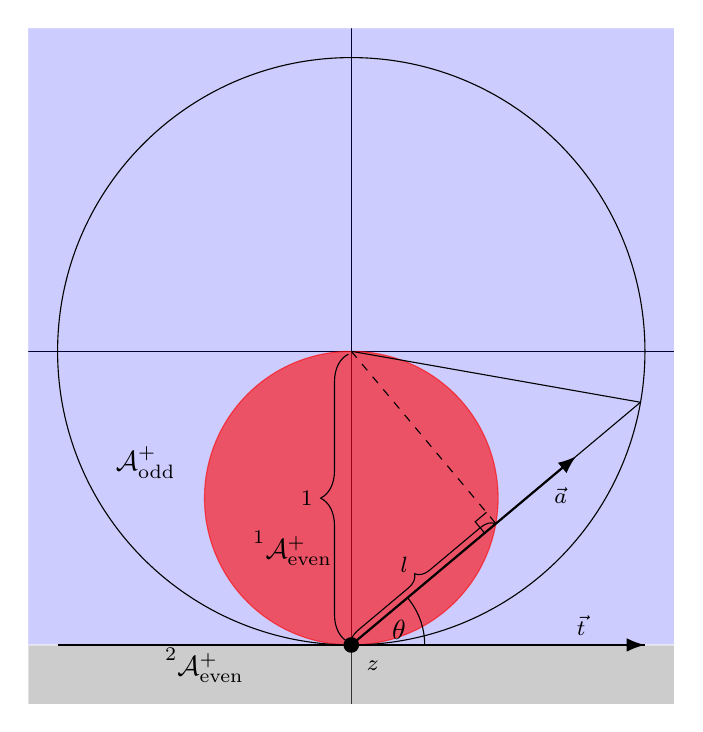
\begin{tikzpicture}
\begin{axis}[ 
    axis lines = middle,
    ticks = none,
    axis line style={-},
    ymin=-1.2, ymax=1.1,
    xmin=-1.1, xmax=1.1,
    axis equal image,
    height=4in
]

\draw[color=white, fill = blue, opacity=0.2] (axis cs:-1.1, -1) rectangle (axis cs:1.1, 1.1);
\draw[color=white, fill = gray, opacity=0.4] (axis cs:-1.1, -1.3) rectangle (axis cs:1.1, -1);

\def\figphi{10}
%p/4-phi/2=theta where phi is angle from x-axis of unit circle to top right point of triangle
\def\figtheta{45-\figphi/2}

\draw[color=black] (axis cs:-1, -1) -- (axis cs:1, -1);
\addplot[data cs=polar, red, opacity=0.6, domain=0:180,samples=180,smooth, fill=red, fill opacity=0.6, shift={(0, transformdirectiony(-1))}] (x, {cos(90 - x)});
\begin{scope}[shift={(0, transformdirectiony(-1))}]
  \node[label={315:{\footnotesize $z$}},circle,fill,inner sep=2pt] at (axis cs:0,0) {};
  \draw (axis cs:0.25,0) arc(0:{\figtheta}:{transformdirectionx(0.25)});
  \node at (axis cs:{0.17*cos(0.5*\figtheta)}, {0.17*sin(0.5*\figtheta)}) {$\theta$};
\end{scope}

\draw (axis cs:0,-1) -- (axis cs:{cos(\figphi)},{-sin(\figphi)});
\draw (axis cs:0, 0) -- (axis cs:{cos(\figphi)},{-sin(\figphi)});
\draw[dashed] (axis cs:0, 0) -- (axis cs:{cos(\figphi)/2},{((-sin(\figphi)-1)/2)});
\begin{scope}[shift={({transformdirectionx(cos(\figphi)/2)},{transformdirectiony((-sin(\figphi)-1)/2)})}, rotate around={\figtheta:(axis cs:0, 0)}]
  \draw (axis cs:-0.05,0)|-(axis cs:0,0.05);
\end{scope}

\draw [decorate,decoration={brace,amplitude=10pt,mirror}] (axis cs:-0.01,-0.01) -- (axis cs:-0.01,{-1+0.01}) node [black,midway,xshift={transformdirectionx(-0.15)}] {\footnotesize $1$};

\draw [decorate,decoration={brace,amplitude=5pt}] (axis cs:0,-1) -- (axis cs:{0.5*cos(\figphi)},{0.5*(-sin(\figphi)-1)}) node [black,midway, xshift={transformdirectionx(-0.07)}, yshift={transformdirectiony(0.07)}] {\footnotesize $l$};

\draw [-Latex, thick] (axis cs:0,-1) -- (axis cs:{cos(\figtheta)},{sin(\figtheta)-1}) node [black,midway, xshift={transformdirectionx(0.35)}, yshift={transformdirectiony(0.2)}] {\footnotesize $\vec{a}$};
  \draw [-Latex, thick] (axis cs:0, -1) -- (axis cs:1, -1) node [black,midway,xshift={transformdirectionx(0.3)},yshift={transformdirectiony(0.07)}] {\footnotesize $\vec{t}$};

\draw (axis cs:0,0) circle [radius=1];

\node[label={{$\prescript{2}{}{\aeven}$}}] at (axis cs:-0.5,-1.2) {};
\node[label={{$\prescript{1}{}{\aeven}$}}] at (axis cs:-0.2,-0.8) {};
\node[label={{$\aodd$}}] at (axis cs:-0.7,-0.5) {};

\end{axis}
\end{tikzpicture}
\end{center}
%:

Notice a disk only intersects $\mathcal{C}$ if $a$ points in the top half plane \& if $r > l$, and notably there is always a single intersection. From the picture we can deduce
$$
l = \sin\theta
$$
so that\footnote{N.B. $b$ is entirely determined by $a, t$ since $a \cdot b = 0, b \cdot t > 0$}:
\begin{IEEEeqnarray*}{rCl}
  \aodd &=& \braces{
    \parens{\begin{pmatrix} \cos\theta \\ \sin\theta\end{pmatrix}, \begin{pmatrix} \sin\theta \\ -\cos\theta \end{pmatrix}, r} \mid \theta \in \bracp{0, \pi}, r \in [\sin \theta, \infty)
  } \\
  \prescript{1}{}{\aeven} &=& \braces{
    \parens{\begin{pmatrix} \cos\theta \\ \sin\theta\end{pmatrix}, \begin{pmatrix} \sin\theta \\ -\cos\theta \end{pmatrix}, r} \mid \theta \in \bracp{0, \pi}, r \in [0, \sin\theta)
  } \\
  \prescript{2}{}{\aeven} &=& \braces{
    \parens{\begin{pmatrix} \cos\theta \\ \sin\theta\end{pmatrix}, \begin{pmatrix} -\sin\theta \\ \cos\theta \end{pmatrix}, r} \mid \theta \in \bracp{\pi, 2\pi}, r \in [0, \infty)
  } \\
  \aeven &=& \prescript{1}{}{\aeven} \cup \prescript{2}{}{\aeven}.
\end{IEEEeqnarray*}
Put $\chi_1 = \chi_{\aeven} - \chi_{\aodd}$ so that we can rewrite our calculation as:
$$
\kappa_\sigma \cdot n = \int_{\aeven \cup \aodd} \frac{\chi_1(r, a)}{r^{1+\sigma}} \parens{(a \cdot t)(b\cdot n) - (b \cdot t)(a \cdot n)} \, d\haus{2}{a,b,r}
$$
Next consider a change of variables via $\phi : [0, 2\pi] \times \mathbb{R}^+ \to \aeven \cup \aodd$ given by
$$
\phi(\theta, r) = \parens{\begin{pmatrix} \cos\theta \\ \sin\theta\end{pmatrix}, \begin{pmatrix} \sin\theta \\ -\cos\theta \end{pmatrix}, r}.
$$
For $\gamma : \mathbb{R} \to [0, 2\pi] \times \mathbb{R}^+$ such that $\gamma(0) = (\theta, r)$ and $\gamma'(0) = (1, 0)$ we find
$$
\left. \dby{s} \phi(\gamma(s)) \right|_{s=0} = \parens{\begin{pmatrix} -\sin \theta \\ \cos \theta \end{pmatrix}, \begin{pmatrix} \cos \theta \\ \sin\theta \end{pmatrix}, 0} = \parens{-b, a, 0}
$$
and similarly when we consider $\gamma$ such that $\gamma'(0) = (0, 1)$ we find:
$$
\left. \dby{s} \phi(\gamma(s)) \right|_{s=0} = \parens{ \begin{pmatrix} 0 \\ 1 \end{pmatrix}, \begin{pmatrix} 1 \\ 0 \end{pmatrix}, 1 } = \parens{b, -a, 0} + \parens{0, 0, 1}.
$$
Since $T_{(a, b, r)} \aeven \cup \aodd$ is spanned by $\frac{1}{\sqrt{2}} (b, -a, 0), (0, 0, 1)$ we can write $\nabla \phi$ as follows:
$$
\nabla \phi (a, b, r) = \begin{blockarray}{ccc}
  (1, 0) & (0, 1) \\
  \begin{block}{(cc)c}
    -\sqrt{2} & 0 & \frac{1}{\sqrt{2}} (b, -a, 0) \\
    0 & 1 & (0, 0, 1)  \\
  \end{block}
\end{blockarray} \implies \sqrt{\abs{\nabla \phi^T \nabla \phi}} = \sqrt{2}.
$$

With this change of variables our computation becomes:
\begin{IEEEeqnarray*}{rCl}
  \kappa_\sigma \cdot n &=&
  \sqrt{2} \int_{[0, 2\pi] \times \mathbb{R}^+}
\frac{\chi_1\parens{r, \begin{pmatrix} \cos \theta \\ \sin \theta \end{pmatrix}}}{r^{1+\sigma}} \parens{- \cos^2 \theta - \sin^2 \theta} \chi_2\parens{r, \begin{pmatrix} \cos \theta \\ \sin\theta \end{pmatrix}}
  \, dr \, d\theta \\
  &=&
  -\sqrt{2} \int_{[0, 2\pi] \times \mathbb{R}^+} \frac{\chi_1\parens{r, \theta}}{r^{1+\sigma}} \chi_2\parens{r, \theta} \, dr \, d\theta \\
\end{IEEEeqnarray*}
where $\chi_2 = \chi_{\prescript{1}{}{\aeven} \cup \aodd} - \chi_{\prescript{2}{}{\aeven}}$. Fix $\chi = \chi_1 \chi_2 = \chi_{\prescript{1}{}{\aeven}} - \chi_{\prescript{2}{}{\aeven} \cup \aodd}$ so that
\begin{IEEEeqnarray*}{rCl}
  \int_{[0, 2\pi] \times \mathbb{R}^+} \frac{\chi_1\parens{r, \theta}}{r^{1+\sigma}} \chi_2\parens{r, \theta} \, dr \, d\theta
    &=&
  \lim_{\epsilon \downarrow 0} \int_0^{2\pi} \int_{\epsilon}^\infty \frac{\chi(r, \theta)}{r^{1+\sigma}} \, dr \, d\theta \\
  &=& \lim_{\epsilon \downarrow 0} \parens{\int_0^\pi \int_\epsilon^{\sin\theta} r^{-1-\sigma} \, dr \, d\theta - \int_0^\pi \int_{\sin \theta}^\infty r^{-1-\sigma} \, dr \, d\theta - \int_\pi^{2\pi} \int_\epsilon^\infty r^{-1-\sigma} \, dr \, d\theta} \\
  &=& \frac{-1}{\sigma} \lim_{\epsilon \downarrow 0} \parens{ \int_0^\pi \left. r^{-\sigma} \right|_{\epsilon}^{\sin \theta} \, d\theta - \int_0^\pi \left. r^{-\sigma} \right|_{\sin \theta}^\infty \, d\theta - \int_\pi^{2\pi} \left. r^{-\sigma} \right|_{\epsilon}^\infty } \\
  &=& \frac{-1}{\sigma} \lim_{\epsilon \downarrow 0} \parens{ \int_0^\pi \sin^{-\sigma} \theta \, d\theta - \pi \epsilon^{-\sigma} + \int_0^\pi \sin^{-\sigma} \theta \, d\theta + \pi \epsilon^{-\sigma} } \\
  &=& \frac{-2}{\sigma} \int_0^\pi \sin^{-\sigma} \theta \, d\theta = \frac{-2}{\sigma} \int_{-\pi / 2}^{\pi / 2} \cos^{-\sigma} \theta \, d\theta = \frac{-4}{\sigma} \int_0^{\pi / 2} \cos^{-\sigma} \theta \, d\theta \\
  &=& \frac{-2}{\sigma} B\parens{\frac{1}{2}, \frac{1-\sigma}{2}} \\
  \implies \kappa_\sigma \cdot n &=& \frac{2^{3/2}}{\sigma} B\parens{\frac{1}{2}, \frac{1-\sigma}{2}}
\end{IEEEeqnarray*}%:

\section{Fractional Curvature of Unit Circle in N-D}%;
To begin, fix $\chi(a,b,r)$ to indicate the sign corresponding to $a, b, r$ (i.e. whether $a, b, r$ belong to $\aeven$ or $\aodd$, and whether $b$ or $-b$ is needed by the $t \cdot b > 0$ restriction). Put $\mathcal{A}^+ = \aeven \cup \aodd$ and
$$
g(a, b, r) = \frac{\parens{\bec{a} \cdot \bec{t}(z)} \bec{b} - \parens{\bec{b} \cdot \bec{t}(z)}\bec{a}}{r^{1+\sigma}},
$$
so that our desired computation is:
$$
\kappa_\sigma(z) = \int_{\mathcal{A}^+} \chi(a, b, r) g(a, b, r) \, d\mathcal{H}^{2n-2}\parens{\bec{a}, \bec{b}, r},
$$

\subsection{Slicing out the 2D plane}%;
To simplify our domain group the disks by their intersection with the $S := \lsp{t, n}$ plane, i.e. put $\psi : \mathcal{A}^+ \to \mathbb{R}^2$ so that $\psi$ maps a disk to a vector representing $\mathcal{D}(a, b, r) \cap S$. The same constraints that applied in 3D above apply once again here, so that, with $p(b) = \frac{\mathcal{P}_S b^\perp}{\abs{\mathcal{P}_S b^\perp}}$ we have
$$
  \psi(a, b, r) = 2r \parens{p(b) \otimes p(b)} a.
$$%:

\subsection{2D Co-Area Calculation}%;

To begin our calculation put $c = \frac{u - \parens{u \cdot a}a}{\sqrt{u \cdot u - \parens{u \cdot a}^2}}$ and $\braces{e_i}_{i=1}^{n-3}$ so that $\lsp{a, b, c, e_1, ..., e_{n-3}} = \mathbb{R}^n$. Notice that
$$
\lsp{a, b, p} = \lsp{a, b, \frac{u}{\abs{u}}} = \lsp{a, b, u} \subset \lsp{a, b, c},
$$
and that $a, b, c$ are orthonormal. Further, we have
$$
T_{(a,b,r)}(\mathcal{U}_\perp^2 \times \mathbb{R}^+) = \lsp{ (e_i, 0, 0), (0, e_i, 0), (c, 0, 0), (0, c, 0), \frac{1}{\sqrt{2}} (b, -a, 0), (0, 0, 1) \mid i = 1, ... (n-3)}.
$$

Put $p = p(b)$ so that $p, p^\perp$ spans $T_{\psi(a,b,r)}(\mathbb{R}^2)$. We start with a quick calculation; suppose $\beta : \mathbb{R} \to \mathcal{U}\parens{\mathbb{R}^n}$ such that $\beta(0) = b$, then
\begin{IEEEeqnarray*}{rCl}
  \left. \dby{s} p(\beta(s)) \right|_{s=0} &=& \frac{\sproj \beta '(0)^\perp}{\abs{\sproj b^\perp}} - \frac{1}{\abs{\sproj b^\perp}^3} \sproj b^\perp \otimes \parens{\sproj \beta '(0)^\perp}^T \sproj b^\perp \\
  &=& \frac{1}{\abs{\sproj b^\perp}} \parens{ \sproj \beta '(0)^\perp - \frac{1}{\abs{\sproj b^\perp}^2} \parens{\sproj \beta '(0)^\perp \cdot \sproj b^\perp} \sproj b^\perp } \\
  &=& \frac{1}{\abs{\sproj b^\perp}} \parens{1 - \parens{p \otimes p}} \sproj \beta '(0)^\perp .
\end{IEEEeqnarray*}

Since we'll be working in the $p, p^\perp$ coordinate system, it makes sense to expand this result as follows:
\begin{equation}
  \left. \dby{s} p(\beta(s)) \right|_{s=0} = \frac{1}{\abs{\sproj b^\perp}} \parens{ p \otimes p + p^\perp \otimes p^\perp - p \otimes p } \sproj \beta '(0)^\perp =
  \frac{\parens{p^\perp \otimes p^\perp}}{\abs{\sproj b^\perp}} \sproj \beta '(0)^\perp \label{npb1}
\end{equation}
Now, put $\gamma_v : \mathbb{R} \to \mathcal{U}_\perp^2 \times \mathbb{R}^+$ to be such that $\gamma_v (0) = (a, b, r)$ and $\gamma_v '(0) = v$, then we begin by computing the derivative along the $\gamma_{(e_i, 0, 0)}$ flow:

\begin{equation}
  \left. \dby{s} \psi(\gamma_{(e_i, 0, 0)}(s)) \right|_{s=0} = 2r \parens{ p \otimes p } e_i = 2r \parens{p \cdot e_i} p = 0. \label{ng1.2}
\end{equation}
Similarly we can compute along the $(c, 0, 0)$ flow:
\begin{equation}
  \left. \dby{s} \psi(\gamma_{(c, 0, 0)}(s)) \right|_{s=0} = 2r \parens{ p \otimes p } e_i = 2r \parens{p \cdot c} p. \label{ng1}
\end{equation}
Next we compute along the $\braces{ (0, v, 0) \mid v = e, e_1, e_2, ..., e_{n-3} }$ flows, and simplify using \eqref{npb1}
\begin{IEEEeqnarray*}{rCl}
  \left. \dby{s} \psi(\gamma_{(0, v, 0)}(s)) \right|_{s=0} &=& 2r \parens{ \parens{ \left. \dby{s}p(\gamma_{(0, v, 0),2}(s))\right|_{s=0} }\otimes p + p \otimes \parens{ \left. \dby{s} p(\gamma_{(0, v, 0),2}(s)) \right|_{s=0} } } a \\
  &=& 2r \parens{ \parens{\frac{\parens{p^\perp \otimes p^\perp}}{\abs{\sproj b^\perp}} \sproj v^\perp} \otimes p + p \otimes \parens{\frac{\parens{p^\perp \otimes p^\perp}}{\abs{\sproj b^\perp}} \sproj v^\perp} }a \\
  &=& 2r \frac{p^\perp \cdot \sproj v^\perp}{\abs{\sproj b^\perp}} \parens{ p^\perp \otimes p + p \otimes p^\perp }a .
\end{IEEEeqnarray*}
Taking into account the fact that $p^\perp \cdot \sproj v^\perp = p \cdot \sproj v = p \cdot v$, and expanding the tensor products we find
\begin{equation}
  \left. \dby{s} \psi(\gamma_{(0, v, 0)}(s)) \right|_{s=0} = 2r \frac{\parens{p \cdot v} \parens{ p^\perp \cdot a}}{\abs{\sproj b^\perp}} p + 2r \frac{\parens{p \cdot v} \parens{ p \cdot a}}{\abs{\sproj b^\perp}} p^\perp . \label{ng2}
\end{equation}
Notably, when $v = e_i$ we have
$$
\left. \dby{s} \psi(\gamma_{(0, e_i, 0)}(s)) \right|_{s=0} = 0.
$$

The next derivative we must compute is along the $\frac{1}{\sqrt{2}} (b, -a, 0)$ flow:
\begin{IEEEeqnarray*}{rCl}
  \left. \dby{s} \psi(\gamma_{\frac{1}{\sqrt{2}}(b, -a, 0)}(s)) \right|_{s=0} &=& \sqrt{2}r \parens{ p \otimes p } b + 2r \parens{ \parens{ \left. \dby{s}p(\gamma_{\frac{1}{\sqrt{2}}(b, -a, 0),2}(s))\right|_{s=0} } \odot p } a \\
  &=& 2r \parens{ \parens{\frac{\parens{p^\perp \otimes p^\perp}}{\abs{\sproj b^\perp}} \sproj \frac{-a}{\sqrt{2}}^\perp} \otimes p + p \otimes \parens{\frac{\parens{p^\perp \otimes p^\perp}}{\abs{\sproj b^\perp}} \sproj \frac{-a}{\sqrt{2}}^\perp} }a \\
  &=& -\sqrt{2}r \frac{p^\perp \cdot \sproj a^\perp}{\abs{\sproj b^\perp}} \parens{ p^\perp \otimes p + p \otimes p^\perp }a .
\end{IEEEeqnarray*}
Note that the first term vanishes because $p \cdot b = 0$. Again taking into account the fact that $p^\perp \cdot \sproj a^\perp = p \cdot \sproj a = p \cdot a$, and expanding the tensor products we find
\begin{equation}
  \left. \dby{s} \psi(\gamma_{\frac{1}{\sqrt{2}}(b, -a, 0)}(s)) \right|_{s=0} = -\sqrt{2}r \frac{\parens{p \cdot a} \parens{ p^\perp \cdot a}}{\abs{\sproj b^\perp}} p - \sqrt{2}r \frac{\parens{p \cdot a}^2}{\abs{\sproj b^\perp}} p^\perp . \label{ng3}
\end{equation}
Lastly computing the derivative through the $(0, 0, 1)$ flow we have:
\begin{equation}
  \left. \dby{s} \psi(\gamma_{(0, 0, 1)}(s)) \right|_{s=0} = 2 \parens{ p \otimes p } a = 2\parens{p \cdot a} p \label{ng4}
\end{equation}

Combining \eqref{ng1}, \eqref{ng2}, \eqref{ng3}, \eqref{ng4} we have
$$
\nabla \psi (a, b, r) = \begin{blockarray}{ccccccc}
  (e_i, 0, 0) & (0, e_i, 0) & (c, 0, 0) & (0, c, 0) & \frac{1}{\sqrt{2}}(b, -a, 0) & (0, 0, 1) \\
  \begin{block}{(cccccc)c}
    0 & 0 &
    2r \parens{p \cdot c} &
    2r \frac{\parens{p \cdot c} \parens{ p^\perp \cdot a}}{\abs{\sproj b^\perp}} &
    -\sqrt{2}r \frac{\parens{p \cdot a} \parens{ p^\perp \cdot a}}{\abs{\sproj b^\perp}} &
    2\parens{p\cdot a} & p \\
    0 & 0 &
    0 &
    2r \frac{\parens{p \cdot c} \parens{ p \cdot a}}{\abs{\sproj b^\perp}} &
    -\sqrt{2}r \frac{\parens{p \cdot a}^2}{\abs{\sproj b^\perp}} &
    0 & p^\perp \\
  \end{block}
\end{blockarray}
$$
Notably the jacobian factor is identical to the jacobian factor in 3D, so we have
$$
J\psi(a, b, r) = \sqrt{\abs{\nabla \psi (a, b, r)^T \nabla \psi (a, b, r)}} =
2\sqrt{2} r \abs{\frac{p \cdot a}{\sproj b^\perp}} \sqrt{2 \parens{p \cdot c}^2 + \parens{p \cdot a}^2}\sqrt{r^2 \parens{p \cdot c}^2 + \parens{p \cdot a}^2} .
$$

Put $\mathcal{D}(u) := \psi^{-1}(\braces{u}), p = p(b)$ so that
\begin{IEEEeqnarray*}{rCl}
  \kappa_\sigma
  &=& \int_{\mathbb{R}^2} \int_{\mathcal{D}(u)} \frac{\chi(a, b, r)g(a, b, r)}{J\psi(a, b, r)} \, d\mathcal{H}^{2n-4}(a, b, r) d\mathcal{H}^2(u) \\
  &=& \int_{\mathbb{R}^2} \chi(u) \int_{\mathcal{D}(u)}
  \frac{g(a, b, r)}{2\sqrt{2} r \abs{\frac{p \cdot a}{\sproj b^\perp}} \sqrt{2 \parens{p \cdot c}^2 + \parens{p \cdot a}^2}\sqrt{r^2 \parens{p \cdot c}^2 + \parens{p \cdot a}^2}}
  \, d\mathcal{H}^{2n-4}(a, b, r) d\mathcal{H}^2(u).
\end{IEEEeqnarray*}
Notably, $\chi(a, b, r) = \chi(\psi(a, b, r)) = \chi(u)$, since the number of intersections only depends on how the $u$ cord intersects $S$\footnote{TODO: reason about the sign of $b$ only depends on this cord, too (since that was built into $\chi(a, b, r)$).}.
%:

\subsection{Focusing on the Normal Component}%;

We claim $\parens{n \otimes n} \kappa_\sigma = \kappa_\sigma$, i.e. $\kappa_\sigma$ only has a component in the $n$ direction. Firstly, notice
$$
g(a, b, r) \cdot t = \frac{\parens{a \cdot t} \parens{b \cdot t} - \parens{b \cdot t} \parens{a \cdot t}}{r^{1+\sigma}} = 0,
$$
so that $\kappa_\sigma$ has no $t$ component. Put
$$
J(a, b, r) = 
  \frac{g(a, b, r)}{2\sqrt{2} r \abs{\frac{p \cdot a}{\sproj b^\perp}} \sqrt{2 \parens{p \cdot c}^2 + \parens{p \cdot a}^2}\sqrt{r^2 \parens{p \cdot c}^2 + \parens{p \cdot a}^2}},
$$
suppose $m \in \mathcal{U}\parens{\braces{n, t}^\perp}$ and consider $R_m = I - 2(m \otimes m)$, an operator which reflects the $m$ component. We wish to show
$$
J(R_m a, R_m b, r) \cdot m = -J(a, b, r) \cdot m,
$$
and that $(a, b, r) \in \mathcal{D}(u) \iff (R_m a, R_m b, r) \in \mathcal{D}(u)$ so that we can conclude $\kappa_\sigma \cdot m$ vanishes as it's an integral of an odd function over a symmetric domain. To that end, we see
$$
\sproj R_m b = \sproj b \implies p(R_m b) = p(b) \implies \parens{ J(R_m a, R_m b, r) \cdot m = - J(a, b, r) \cdot m \iff g(R_m a, R_m b, r) \cdot m = -g(a, b, r) \cdot m}.
$$
We also see
$$
  \psi(R_m a, R_m b, r) = 2r \parens{p(b) \otimes p(b)} \parens{a - 2\parens{m \otimes m}a} = 2r \parens{p(b) \cdot \parens{a - 2\parens{m \cdot a}m}} p(b) = 2r \parens{p(b) \cdot a} p(b) = \psi(a, b, r),
$$
so that, indeed, $(a, b, r) \in \mathcal{D}(u) \iff (R_m a, R_m b, r) \in \mathcal{D}(u)$. Finally
\begin{IEEEeqnarray*}{rCl}
  r^{1+\sigma} g(R_m a, R_m b, r) \cdot m &=& \parens{R_m a \cdot t}\parens{R_m b \cdot m} - \parens{R_m b \cdot t}\parens{R_m a \cdot m} \\
  &=& \parens{\parens{a - 2\parens{m \cdot a}m} \cdot t} \parens{R_m b \cdot m} - \parens{R_m b \cdot t}\parens{ \parens{a - 2\parens{m \cdot a}m} \cdot m } \\
  &=& \parens{a \cdot t} \parens{R_m b \cdot m} - \parens{R_m b \cdot t} \parens{\parens{a \cdot m} - 2\parens{m \cdot a}} \\
  &=& \parens{a \cdot t} \parens{ \parens{b - 2\parens{m \cdot b}m} \cdot m} + \parens{\parens{b - 2\parens{m \cdot b}m} \cdot t} \parens{m \cdot a} \\
  &=& \parens{a \cdot t} \parens{\parens{b \cdot m} - 2\parens{m \cdot b}} + \parens{b \cdot t} \parens{m \cdot a} \\
  &=& -\parens{a \cdot t} \parens{b \cdot m} + \parens{b \cdot t}\parens{a \cdot m} \\
  &=& -\parens{\parens{a \cdot t}b - \parens{b \cdot t}a}\cdot m = -r^{1+\sigma} g(a, b, r) \cdot m,
\end{IEEEeqnarray*}
thus our claim is shown and $\kappa_\sigma = \parens{n \otimes n} \kappa_\sigma$, so for the rest of the paper we shall focus on $\kappa_\sigma \cdot n$.
%:

\subsection{Slicing out Radii}%;
Now, to simplify $\mathcal{D}(u)$ lets group sets of $\bec{a}, \bec{b}$ that correspond to a given $r$, i.e. put $\phi : \mathcal{D}(u) \to \mathbb{R}^+$ given by
$$
\phi(a, b, r) = r.
$$

To begin our calculation of $\nabla \phi$ we must characterize $T_{(a, b, r)}(\mathcal{D}(u))$, i.e. via finding an orthonormal basis. Suppose $\gamma : \mathbb{R} \to \mathcal{D}(u)$ is so that $\gamma(0) = (a, b, r)$ and put $(\delta_a, \delta_b, \delta_r) := \gamma'(0)$. Note $\delta_a \cdot a = \delta_b \cdot b = 0$ and $\delta_a \cdot b + a \cdot \delta_b = 0$, since $(a, b) \in \mathcal{U}_2^\perp$. By the definition of $\mathcal{D}(u)$ we know
$$
2r \parens{p(b) \otimes p(b)} a = u,
$$
so that
$$
2\gamma_3(s) \parens{p(\gamma_2(s)) \otimes p(\gamma_2(s))} \gamma_1(s) = u.
$$
Differentiating\footnote{N.B. we use \eqref{npb1}} and evaluating at $s = 0$ we see
$$
  0 = \delta_r \parens{p(b) \otimes p(b)} a + r \parens{\frac{\parens{p^\perp \otimes p^\perp}}{\abs{\mathcal{P}_S b^\perp}} \mathcal{P}_S \delta_b^\perp \odot p(b)} a + r \parens{p(b) \otimes p(b)} \delta_a.
$$
Expanding tensor products, simplifying and using the $p, p^\perp$ coordinate system we get
\begin{IEEEeqnarray*}{rCl}
  0 &=& \delta_r \parens{p \cdot a} p + r\parens{\frac{p \cdot \delta_b}{\abs{\mathcal{P}_S b^\perp}}p^\perp \odot p} a + r \parens{p \cdot \delta_a} p \\
  &=& \parens{\delta_r\parens{p \cdot a} + r \parens{p \cdot \delta_a}}p +
  r \frac{\parens{p \cdot \delta_b}}{\abs{\mathcal{P}_S b^\perp}} \parens{p^\perp \otimes p + p \otimes p^\perp}a \\
  &=& \parens{\delta_r\parens{p \cdot a} + r \parens{p \cdot \delta_a}
  + r \frac{\parens{p \cdot \delta_b}}{\abs{\mathcal{P}_S b^\perp}} \parens{p^\perp \cdot a}}p
  + r \frac{\parens{p \cdot \delta_b}}{\abs{\mathcal{P}_S b^\perp}} \parens{p \cdot a} p^\perp .
\end{IEEEeqnarray*}
Notably, we must have $p \cdot \delta_b = 0$, so our constraint simplifies to
$$
0 = \delta_r \parens{p \cdot a} + r \parens{p \cdot \delta_a}.
$$
Observe $(e_i, 0, 0), (0, e_i, 0)$ are $2n-6$ valid basis vectors abiding by our constraints. Additionally, fixing $\delta_b = 0$ and considering $\delta_a \neq e_i$ (so as to find an additional orthonormal basis vector) we must have $\delta_a = c$, and thus 
$$
\mu = \frac{1}{\sqrt{1 + r^2 \frac{\parens{p\cdot c}^2}{\parens{p \cdot a}^2}}} \parens{c, 0, -r\frac{\parens{p \cdot c}}{\parens{p \cdot a}}},
$$
is an additional basis vector. Put $\mathcal{R}(u, r) = \sqrt{r^2 - \frac{\abs{u}^2}{4}}$ and consider the vector
$$
\nu = \parens{ \frac{\mathcal{R}(u, r)}{\mathcal{R}(u, \sqrt{2}r)} b, \frac{r}{2 \mathcal{R}(u, r) \mathcal{R}(u, \sqrt{2}r)} \parens{u - 2ra}, 0 }.
$$
Observe
\begin{IEEEeqnarray*}{rCl}
  \abs{\nu}^2 &=& \frac{\mathcal{R}^2(u, r)}{\mathcal{R}^2(u, \sqrt{2}r)} + \frac{r^2}{4 \mathcal{R}^2(u, r) \mathcal{R}^2(u, \sqrt{2}r)} \parens{ \abs{u}^2 + 4r^2 - 4r \parens{u \cdot a} } \\
  &=& \frac{\mathcal{R}^2(u, r)}{\mathcal{R}^2(u, \sqrt{2}r)} + \frac{r^2}{4 \mathcal{R}^2(u, r) \mathcal{R}^2(u, \sqrt{2}r)} \parens{ \abs{u}^2 + 4r^2 - 4r \frac{\abs{u}^2}{2r} } \\
  &=& \frac{\mathcal{R}^2(u, r)}{\mathcal{R}^2(u, \sqrt{2}r)} + \frac{r^2}{4\mathcal{R}^2(u, r) \mathcal{R}^2(u, \sqrt{2}r)} \parens{4r^2 - \abs{u}^2} \\
  &=& \frac{\mathcal{R}^2(u, r)}{\mathcal{R}^2(u, \sqrt{2}r)} + \frac{r^2}{\mathcal{R}^2(u, \sqrt{2}r)} = 1,
\end{IEEEeqnarray*}
so that $\nu$ is the final basis vector spanning $T_{(a, b)} \mathcal{D}(u)$. Now, to compute $J \phi$, for $v \in \{\mu,\nu\}$, put $\gamma_v : \mathbb{R} \to \mathcal{D}(u)$ so that $\gamma_v(0) = (a, b, r)$ and $\gamma'(0) = v$. Then we have a few trivial derivatives:
\begin{IEEEeqnarray*}{rCl}
  \left. \dby{s} \phi(\gamma_{(e_i, 0, 0)}(s)) \right|_{s=0} &=& 0. \\
  \left. \dby{s} \phi(\gamma_{(0, e_i, 0)}(s)) \right|_{s=0} &=& 0. \\
  \left. \dby{s} \phi(\gamma_\nu(s)) \right|_{s=0} &=& 0,
\end{IEEEeqnarray*}
Now we're able to compute the derivative along the non-trivial flow
\begin{IEEEeqnarray*}{rCl}
  \left. \dby{s} \phi(\gamma_\mu(s)) \right|_{s=0} &=& \frac{-r \parens{p \cdot c}}{\parens{p \cdot a} \sqrt{1 + r^2 \frac{\parens{p\cdot c}^2}{\parens{p\cdot a}^2}}} \\
  &=& -r\frac{\parens{p \cdot c}}{\sqrt{\parens{p\cdot a}^2 + r^2 \parens{p \cdot c}^2}} \\
\end{IEEEeqnarray*}
so that
$$
J \phi = \frac{r \abs{p \cdot c}}{\sqrt{\parens{p \cdot a}^2 + r^2 \parens{p \cdot c}^2}}.
$$

Put $\mathcal{D}(u, r) = \phi^{-1}(\{r\})$ so that our top-level calculation becomes

\begin{IEEEeqnarray*}{ll}
  &\int_{\mathbb{R}^2} \chi(u) \int_{\mathcal{D}(u)} \frac{g(a, b, r) \cdot n}{2\sqrt{2} r \abs{\frac{p \cdot a}{\sproj b^\perp}} \sqrt{2 \parens{p \cdot c}^2 + \parens{p \cdot a}^2}\sqrt{r^2 \parens{p \cdot c}^2 + \parens{p \cdot a}^2}} \, d\mathcal{H}^{2n-4}(a, b, r) d\mathcal{H}^2(u) \\
  &= \int_{\mathbb{R}^2} \chi(u) \int_{\phi(\mathcal{D}(u))} \int_{\mathcal{D}(u, r)}
  \frac{g(a, b, r) \cdot n}{2\sqrt{2} r \abs{\frac{p \cdot a}{\sproj b^\perp}} \sqrt{2 \parens{p \cdot c}^2 + \parens{p \cdot a}^2}\sqrt{r^2 \parens{p \cdot c}^2 + \parens{p \cdot a}^2}}
  \frac{\sqrt{\parens{p\cdot a}^2 + r^2 \parens{p \cdot c}^2}}{r \abs{p \cdot c}}
  \, d\mathcal{H}^{2n-5}(a, b) dr d\mathcal{H}^2(u) \\
  &= \int_{\mathbb{R}^2} \chi(u) \int_{\phi(\mathcal{D}(u))} \int_{\mathcal{D}(u, r)} \frac{\parens{g(a, b, r) \cdot n} \abs{\sproj b^\perp}}{2\sqrt{2} \abs{\parens{p \cdot a}\parens{p \cdot c}} r^2 \sqrt{2 \parens{p \cdot c}^2 + \parens{p \cdot a}^2}}
  \, d\mathcal{H}^{2n-5}(a, b) dr d\mathcal{H}^2(u)
\end{IEEEeqnarray*}
%:

\subsection{Simplifying Computation}%;
In order to simplify our calculation recall
$$
g(a, b, r) = \frac{\parens{a \cdot t}b - \parens{b \cdot t}a}{r^{1+\sigma}}.
$$
Now, from \ref{perpdef} we see 
$$
  \parens{a \cdot t} \parens{b \cdot n} - \parens{b \cdot t} \parens{a \cdot n} = - \sproj b^\perp \cdot a = - \abs{\sproj b^\perp} \parens{p \cdot a},
$$
so
$$
g(a, b, r) \cdot n = \frac{\parens{a \cdot t} \parens{b \cdot n} - \parens{b \cdot t} \parens{a \cdot n}}{r^{1+\sigma}} = -\frac{\abs{\sproj b^\perp} \parens{p \cdot a}}{r^{1+\sigma}}.
$$
We also know $p \in \lsp{a, b, c}$ so that
$$
\parens{p \cdot a}^2 + \parens{p \cdot b}^2 + \parens{p \cdot c}^2 = \abs{p} = 1 \implies \abs{p \cdot c} = \sqrt{1- \parens{p \cdot a}^2}.
$$
And finally, before simplifying our integrand let's note that
$$
2r \parens{p \cdot a} p = u \implies \abs{u} = 2r\parens{p \cdot a} \implies \parens{p \cdot a} = \frac{\abs{u}}{2r},
$$
and in particular this means $p \cdot a > 0$. Altogether, substituting this into our integrand we see
\begin{IEEEeqnarray*}{rCl}
  \frac{1}{2\sqrt{2}}\frac{1}{r^2} \abs{\frac{\sproj b^\perp}{\parens{p \cdot a}\parens{p \cdot c}}} \frac{g(a, b, r) \cdot n}{\sqrt{2\parens{p \cdot c}^2 + \parens{p\cdot a}^2}} &=& \frac{-1}{2\sqrt{2}} \frac{1}{r^{3+\sigma}} \frac{\abs{\sproj b^\perp}^2 \parens{p \cdot a}}{\parens{p \cdot a}\abs{p \cdot c}} \frac{1}{\sqrt{2 \parens{p \cdot c}^2 + \parens{p \cdot a}^2}} \\
  &=& \frac{-1}{2\sqrt{2}} \frac{1}{r^{3+\sigma}} \frac{\abs{\sproj b^\perp}^2}{\sqrt{1-\parens{p \cdot a}^2} \sqrt{2-\parens{p \cdot a}^2}} \\
  &=& \frac{-1}{2\sqrt{2}} \frac{1}{r^{3+\sigma}} \frac{\abs{\sproj b^\perp}^2}{\sqrt{1-\frac{\abs{u}^2}{4r^2}}\sqrt{2-\frac{\abs{u}^2}{4r^2}}} \\
  &=& \frac{-1}{2\sqrt{2}} \frac{1}{r^{1+\sigma}} \frac{\abs{\sproj b^\perp}^2}{\mathcal{R}(u, r) \mathcal{R}(u, \sqrt{2}r)}.
\end{IEEEeqnarray*}

Thus, putting this back into our integral we find
\begin{IEEEeqnarray*}{rCl}
  \kappa_\sigma \cdot n &=&
  \int_{\mathbb{R}^2} \chi(u) \int_{\phi(\mathcal{D}(u))} \int_{\mathcal{D}(u, r)}
  \frac{-1}{2\sqrt{2}} \frac{1}{r^{1+\sigma}} \frac{\abs{\sproj b^\perp}^2}{\mathcal{R}(u, r) \mathcal{R}(u, \sqrt{2}r)}
  \, d\mathcal{H}^{2n-5}(a, b) dr d\mathcal{H}^2(u) \\
  &=&
  \frac{-1}{2\sqrt{2}} \int_{\mathbb{R}^2} \chi(u) \int_{\phi(\mathcal{D}(u))} \frac{1}{r^{1+\sigma} \mathcal{R}(u, r) \mathcal{R}(u, \sqrt{2}r)} \int_{\mathcal{D}(u, r)} \abs{\sproj b^\perp}^2
  \, d\mathcal{H}^{2n-5}(a, b) dr d\mathcal{H}^2(u)
\end{IEEEeqnarray*}%:

\subsection{Splitting Spheres}%;

In order to compute the inner most integral we will apply the co-area formula once again to slice out all $\mathcal{B}(u) = \braces{ b \in \mathcal{U}\parens{\braces{u}^\perp} \mid b \cdot t > 0 }$, i.e. the projection of $\mathcal{D}(u, r)$ onto the $b$ coordinates. Concretely, our slicing function $\xi : \mathcal{D}(u, r) \to \mathcal{B}(u)$ is given by $\xi(a, b) = b$. From our above calculations we know
$$
T_{(a, b)} \mathcal{D}(u, r) = \lsp{ (e_i, 0), (0, e_i), \nu },
$$
where, for $\mathcal{R}(u, r) = \sqrt{r^2 - \frac{\abs{u}^2}{4}}$, we put
$$
\nu = \parens{ \frac{\mathcal{R}(u, r)}{\mathcal{R}(u, \sqrt{2}r)} b, \frac{r}{2 \mathcal{R}(u, r) \mathcal{R}(u, \sqrt{2}r)} \parens{u - 2ra} }.
$$
Similarly, we know\footnote{N.B. We're able to use $e_i, a$ in our basis because $a$ is fixed for this calculation.} $T_b \mathcal{B}(u) = \lsp{ e_i, \frac{\nu_2}{\abs{\nu_2}} }$ and so we can compute
$$
\nabla \xi (a, b) =
\begin{blockarray}{cccc}
  (e_i, 0) & (0, e_i) & \nu &\\
  \begin{block}{(ccc)c}
    0 & I & 0 & e_i \\
    0 & 0 & \abs{\nu_2} & \frac{\nu_2}{\abs{\nu_2}} \\
  \end{block}
\end{blockarray}
  \implies \nabla \xi (a, b) \parens{\nabla \xi (a, b)}^T = 
\begin{blockarray}{ccc}
  \overbrace{}^{n-3} & \overbrace{}^{1} &\\
  \begin{block}{(cc)c}
    I  & 0 & {\scriptstyle n-3} \\
    0 & \abs{\nu_2}^2 & {\scriptstyle 1} \\
  \end{block}
\end{blockarray}.
$$
This tells us
\begin{IEEEeqnarray*}{rCl}
  J \xi(a, b) &=& \abs{\nu_2} = \sqrt{\frac{r^2}{4\mathcal{R}^2(u, r) \mathcal{R}^2(u, \sqrt{2}r)} \parens{ \abs{u}^2 + 4r^2 - 4 r \parens{u \cdot a} }} \\
  &=& \sqrt{\frac{r^2}{4\mathcal{R}^2(u, r) \mathcal{R}^2(u, \sqrt{2}r)} \parens{ \abs{u}^2 + 4r^2 - 4r \frac{\abs{u}^2}{2r} }} \\
  &=& \sqrt{\frac{r^2}{4\mathcal{R}^2(u, r) \mathcal{R}^2(u, \sqrt{2}r)} \parens{ 4r^2 - \abs{u}^2 }} \\
  &=& \sqrt{\frac{r^2}{4\mathcal{R}^2(u, r) \mathcal{R}^2(u, \sqrt{2}r)} 4 \mathcal{R}^2(u, r)} \\
  &=& \sqrt{\frac{r^2}{\mathcal{R}^2(u, \sqrt{2}r)}} = \frac{r}{\mathcal{R}(u, \sqrt{2}r)}.
\end{IEEEeqnarray*}
Putting $\mathcal{A}(u, r, b) = \xi^{-1}(\braces{b})$ and plugging this back into our desired calculation we find
\begin{IEEEeqnarray*}{rCl}
  \kappa_\sigma \cdot n &=& 
  \frac{-1}{2\sqrt{2}} \int_{\mathbb{R}^2} \chi(u) \int_{\phi(\mathcal{D}(u))} \frac{1}{r^{1+\sigma} \mathcal{R}(u, r) \mathcal{R}(u, \sqrt{2}r)} \int_{\mathcal{B}(u)} \abs{\sproj b^\perp}^2
  \int_{\mathcal{A}(u, r, b)} \frac{1}{J \xi(a, b)} \, d \haus{n-3}{a} \, d \haus{n-2}{b} \, dr \, d \haus{2}{u} \\
  &=& 
  \frac{-1}{2\sqrt{2}} \int_{\mathbb{R}^2} \chi(u) \int_{\phi(\mathcal{D}(u))} \frac{\mathcal{R}(u, \sqrt{2}r)}{r^{2+\sigma} \mathcal{R}(u, r) \mathcal{R}(u, \sqrt{2}r)} \int_{\mathcal{B}(u)} \abs{\sproj b^\perp}^2
  \int_{\mathcal{A}(u, r, b)} \, d \haus{n-3}{a} \, d \haus{n-2}{b} \, dr \, d \haus{2}{u} \\
  &=&
  \frac{-1}{2\sqrt{2}} \int_{\mathbb{R}^2} \chi(u) \int_{\phi(\mathcal{D}(u))} \frac{1}{r^{2+\sigma} \mathcal{R}(u, r) } \int_{\mathcal{B}(u)} \abs{\sproj b^\perp}^2
  \int_{\mathcal{A}(u, r, b)} \, d \haus{n-3}{a} \, d \haus{n-2}{b} \, dr \, d \haus{2}{u} \\
\end{IEEEeqnarray*}

%:

\subsection{Inner Sphere Volume}%;
We begin by seeing
$$
\parens{a - \frac{u}{2r}} \cdot \parens{a - \frac{u}{2r}} = 1 + \frac{\abs{u}^2}{4r^2} - 2 \frac{\parens{a \cdot u}}{2r} = 1 + \frac{\abs{u}^2}{4r^2} - 2\frac{\abs{u}^2}{4r^2} = 1 - \frac{\abs{u}^2}{4r^2},
$$
thus we're able to rewrite our sphere as
$$
\mathcal{A}(u, r, b) = \braces{ a \in \mathcal{U}\parens{\braces{b}^\perp} \mid \abs{a - \frac{u}{2r}}^2 = 1 - \frac{\abs{u^2}}{4r^2} }.
$$
This is an $n-3$ dimensional sphere located at $\frac{u}{2r}$ with radius $\sqrt{1 - \frac{\abs{u}^2}{4r^2}}$ and thus we have
$$
  \int_{\mathcal{A}(u, r, b)} \, d \haus{n-3}{a} = \haus{n-3}{\mathcal{A}(u, r, b)} = S_{n-3}\parens{\sqrt{1 - \frac{\abs{u}^2}{4r^2}}}
  = \omega_{n-3} \parens{1 - \frac{\abs{u^2}}{4r^2}}^{(n-3)/2}
  =
  \omega_{n-3} \frac{1}{r^{n-3}} \mathcal{R}^{n-3}(u, r),
$$
where $\omega_{n-1} = \frac{2\pi^{n/2}}{\Gamma(n/2)}$ is the surface area of a unit ball in $\mathbb{R}^n$.

Putting this back into our top-level integral gives us
\begin{IEEEeqnarray*}{ll}
  \frac{-1}{2\sqrt{2}} \int_{\mathbb{R}^2} & \chi(u) \int_{\phi(\mathcal{D}(u))} \frac{1}{r^{2+\sigma} \mathcal{R}(u, r) } \int_{\mathcal{B}(u)} \abs{\sproj b^\perp}^2
  \int_{\mathcal{A}(u, r, b)} \, d \haus{n-3}{a} \, d \haus{n-2}{b} \, dr \, d \haus{2}{u} \\
  &= \frac{-1}{2\sqrt{2}} \int_{\mathbb{R}^2} \chi(u) \int_{\phi(\mathcal{D}(u))} \frac{1}{r^{2+\sigma} \mathcal{R}(u, r) } \int_{\mathcal{B}(u)} \abs{\sproj b^\perp}^2 
  \omega_{n-3} \frac{1}{r^{n-3}} \mathcal{R}^{n-3}(u, r) \, d \haus{n-2}{b} \, dr \, d \haus{2}{u} \\
  &= \frac{-\omega_{n-3}}{2\sqrt{2}} \int_{\mathbb{R}^2} \chi(u) \int_{\phi(\mathcal{D}(u))} \frac{\mathcal{R}^{n-4}(u, r)}{r^{\sigma+n-1} } \int_{\mathcal{B}(u)} \abs{\sproj b^\perp}^2 
  \, d \haus{n-2}{b} \, dr \, d \haus{2}{u}. \\
\end{IEEEeqnarray*}
%:

\subsection{Outer Sphere Volume}%;

First, we have
$$
0 < b \cdot t = \parens{b \cdot \frac{u}{\abs{u}}} \parens{t \cdot \frac{u}{\abs{u}}} + \parens{b \cdot \frac{u^\perp}{\abs{u^\perp}}} \parens{t \cdot \frac{u^\perp}{\abs{u^\perp}}} = \parens{b \cdot \frac{u^\perp}{\abs{u^\perp}}} \parens{t \cdot \frac{u^\perp}{\abs{u^\perp}}},
$$
and so we only care about $b$ s.t. $\mathrm{sgn} \parens{b \cdot \frac{u^\perp}{\abs{u^\perp}}} = \mathrm{sgn} \parens{ t \cdot \frac{u^\perp}{\abs{u^\perp}} }$. Next, put $\zeta : \mathcal{B}(u) \to [-1, 1]$ given by
$$
  \zeta(b) = b \cdot \frac{u^\perp}{\abs{u^\perp}}.
$$
Now, since
$
\mathbb{R}^n = \lsp{\frac{u}{\abs{u}}, \frac{u^\perp}{\abs{u^\perp}}, f_1, f_2, \ldots, f_{n-2}},
$
for some orthonormal $\braces{f_i}$, we have
$$
  \zeta(b)^2 + \parens{b \cdot f_1}^2 + \parens{b \cdot f_2}^2 + \cdots + \parens{b \cdot f_{n-2}}^2 = 1 \implies \parens{b \cdot f_1}^2 + \parens{b \cdot f_2}^2 + \cdots + \parens{b \cdot f_{n-2}}^2 = 1 - \zeta(b)^2,
$$
thus
$$
\zeta^{-1}\parens{\braces{v}} = \braces{ b \in \mathcal{B}(u) \mid b \cdot \frac{u^\perp}{\abs{u^\perp}} = v, \, \parens{b \cdot f_1}^2 + \parens{b \cdot f_2}^2 + \cdots + \parens{b \cdot f_{n-2}}^2 = 1-v^2 },
$$
and so
$$
\int_{\zeta^{-1}(v)} \, d\haus{n-3}{x} = \haus{n-3}{\zeta^{-1}(v)} = \haus{n-3}{S_{n-3}\parens{\sqrt{1-v^2}}} = \omega_{n-3}\parens{1-v^2}^{(n-3)/2}.
$$
In order to apply the co-area formula we also need to compute $J \zeta$. To that end, notice $\mathbb{R}^n = \lsp{\frac{u}{\abs{u}}, b, u^*, g_1, \ldots, g_{n-3}}$ when
$$
u^* = \frac{\frac{u^\perp}{\abs{u^\perp}} - \parens{b \cdot \frac{u^\perp}{\abs{u^\perp}}} b}{\sqrt{1-\parens{b \cdot \frac{u^\perp}{\abs{u^\perp}}}^2}}, \, \braces{g_i} \text{ orthonormal.}
$$
Since $b \in \mathcal{B}(u) \implies \abs{b} = 1, \, b \cdot u = 0$ we must have $\delta_b \cdot b = 0, \, \delta_b \cdot u = 0$, and so
$$
T_b(\mathcal{B}(u)) = \lsp{u^*, g_1, \ldots g_{n-3}}.
$$
With this characterization we're able to see
$$
\nabla \zeta(b) =
\begin{blockarray}{ccccc}
  u^* & g_1 & \ldots & g_{n-3} \\
  \begin{block}{(cccc)c}
    \sqrt{1-\parens{b \cdot \frac{u^\perp}{\abs{u^\perp}}}^2}  & 0 & \cdots & 0 & 1 \\
  \end{block}
\end{blockarray} \implies J \zeta(b) = \sqrt{1-\parens{b \cdot \frac{u^\perp}{\abs{u^\perp}}}^2}.
$$
Lastly, before applying the co-area formula, notice
$$
\abs{\sproj b^\perp} = \abs{\parens{\parens{b \cdot \frac{u}{\abs{u}}} \frac{u}{\abs{u}} + \parens{b \cdot \frac{u^\perp}{\abs{u^\perp}}} \frac{u^\perp}{\abs{u^\perp}}}^\perp} = \abs{b \cdot \frac{u^\perp}{\abs{u^\perp}}}
$$
Now we're ready to finally apply the co-area formula to see
\begin{IEEEeqnarray*}{rCl}
  \int_{\mathcal{B}(u)} \abs{\sproj b^\perp}^2 \, d\haus{n-2}{b} &=&
  \int_{\zeta(\mathcal{B}(u))} \abs{v}^2 \int_{\zeta^{-1}\parens{\braces{v}}} \frac{1}{\sqrt{1-v^2}}\, d\haus{n-3}{x} \, dv \\
  &=&
  \int_{\zeta(\mathcal{B}(u))} \abs{v}^2 \parens{1-v^2}^{-1/2} \int_{\zeta^{-1}\parens{\braces{v}}} \, d\haus{n-3}{x} \, dv \\
  &=&
  \omega_{n-3} \int_{\zeta(\mathcal{B}(u))} v^2 \parens{1-v^2}^{(n-4)/2} \, dv.
\end{IEEEeqnarray*}
We know $\zeta(\mathcal{B}(u)) = [-1, 0] \lor [0, 1]$ depending on $\mathrm{sgn} \parens{ t \cdot u^\perp }$, and so, since our integrand is even, we have
$$
  \omega_{n-3} \int_{\zeta(\mathcal{B}(u))} v^2 \parens{1-v^2}^{(n-4)/2} \, dv = \omega_{n-3} \int_{0}^1 v^2 \parens{1-v^2}^{(n-4)/2} \, dv.
$$
Finally, transforming from $v^2 \to v$ so that $dv \to \frac{1}{2\sqrt{v}} dv$ we deduce
$$
\omega_{n-3} \int_{0}^1 v^2 \parens{1-v^2}^{(n-4)/2} \, dv = \frac{\omega_{n-3}}{2} \int_{0}^1 v^{1/2} \parens{1-v}^{(n-4)/2} \, dv = \frac{\omega_{n-3}}{2} B\parens{\frac{3}{2}, \frac{n-2}{2}}.
$$
Plugging this back into our top-level calculation gives the following
\begin{IEEEeqnarray*}{ll}
  \frac{-\omega_{n-3}}{2\sqrt{2}} &\int_{\mathbb{R}^2} \chi(u) \int_{\phi(\mathcal{D}(u))} \frac{\mathcal{R}^{n-4}(u, r)}{r^{\sigma+n-1} } \int_{\mathcal{B}(u)} \abs{\sproj b^\perp}^2 
  \, d \haus{n-2}{b} \, dr \, d \haus{2}{u} \\
  &=
  \frac{-\omega_{n-3}^2}{4\sqrt{2}} B\parens{\frac{3}{2}, \frac{n-2}{2}}
  \int_{\mathbb{R}^2} \chi(u) \int_{\phi(\mathcal{D}(u))} \frac{\mathcal{R}^{n-4}(u, r)}{r^{\sigma+n-1} } \, dr \, d\haus{2}{u}.
\end{IEEEeqnarray*}
%:

\subsection{Evaluating Integral over Radii}%;

Our computation simplifies to
$$
\kappa_\sigma \cdot n =
  \frac{-\omega_{n-3}^2}{4\sqrt{2}} B\parens{\frac{3}{2},\frac{n-2}{2}}
  \int_{\mathbb{R}^2} \chi(u) \int_{\frac{\abs{u}}{2}}^\infty r^{1-\sigma-n} \parens{r^2-\frac{\abs{u}^2}{4}}^{(n-4)/2} \, dr \, d\haus{2}{u}.
$$
Using the transformation $r \to \frac{\abs{u}}{2}s^{-1/2} \implies dr = \frac{-\abs{u}}{4}s^{-3/2} ds$ and $r \to \abs{u}/2 \implies s \to 1, \, r \to \infty \implies s \to 0$ we find
\begin{IEEEeqnarray*}{rCl}
  \int_{\frac{\abs{u}}{2}}^\infty r^{1-\sigma-n} \parens{r^2-\frac{\abs{u}^2}{4}}^{(n-4)/2} \, dr &=& \parens{\frac{\abs{u}}{2}}^{1-\sigma-n} \int_0^1 s^{(n+\sigma-1)/2} \parens{\frac{\abs{u}^2}{4} \frac{1}{s} - \frac{\abs{u}^2}{4}}^{(n-4)/2} \frac{\abs{u}}{4} s^{-3/2} ds \\
  &=& \frac{\abs{u}^{2-\sigma-n}}{2^{3-\sigma-n}} \parens{\frac{\abs{u}}{2}}^{n-4} \int_0^1 s^{(n+\sigma-4)/2} \parens{\frac{1-s}{s}}^{(n-4)/2} \, ds \\
  &=& \frac{\abs{u}^{-\sigma-2}}{2^{-\sigma-1}} \int_0^1 s^{\sigma/2} \parens{1-s}^{(n-4)/2} \, ds \\
  &=& \frac{2^{1+\sigma}}{\abs{u}^{2+\sigma}} B\parens{ \frac{\sigma+2}{2}, \frac{n-2}{2} }.
\end{IEEEeqnarray*}
Plugging this back into the above integral we find
$$
\kappa_\sigma \cdot n = -2^{\sigma-3/2}\omega_{n-3}^2 B\parens{\frac{3}{2},\frac{n-2}{2}} B\parens{ \frac{\sigma+2}{2}, \frac{n-2}{2} }
\int_\mathbb{R^2} \frac{\chi(u)}{\abs{u}^{2+\sigma}} \, d\haus{2}{u}.
$$
Just as with the 3D calculation, we're able to convert to polar coordinates and reuse the 2D calculation to find
$$
\kappa_\sigma \cdot n = \frac{\omega_{n-3}^2}{\pi}  B\parens{\frac{3}{2},\frac{n-2}{2}} \frac{\pi2^{\sigma-1/2}}{\sigma} B\parens{ \frac{\sigma+2}{2}, \frac{n-2}{2} } B\parens{\frac{1}{2}, \frac{1-\sigma}{2}}.
$$

%:

%:

\section{Appendix}%;

\subsection{Non-Local Curvature in 3D}%;
To begin, fix $\chi(a,b,r)$ to indicate the sign corresponding to $a, b, r$ (i.e. whether $a, b, r$ belong to $\aeven$ or $\aodd$, and whether $b$ or $-b$ is needed by the $t \cdot b > 0$ restriction). Put $\mathcal{A}^+ = \aeven \cup \aodd$ and
$$
g(a, b, r) = \chi(a, b, r) \frac{\parens{\bec{a} \cdot \bec{t}(z)} \bec{b} - \parens{\bec{b} \cdot \bec{t}(z)}\bec{a}}{r^{1+\sigma}},
$$
so that our desired computation is:
$$
\kappa_\sigma(z) = \int_{\mathcal{A}^+} g(a, b, r) \, d\mathcal{H}^{4}\parens{\bec{a}, \bec{b}, r},
$$

\subsubsection{Slicing out the 2D plane}%;
To simplify our domain group the disks by their intersection with the $S := \lsp{t, n}$ plane, i.e. put $\psi : \mathcal{A}^+ \to \mathbb{R}^2$ so that $\psi$ maps a disk to a vector representing $\mathcal{D}(a, b, r) \cap S$. To determine $\psi$, put $u := \psi(a, b, r)$, then we must have the following:
\begin{itemize}
  \item The component of $ra$ in the direction of $u$ must be half of $u$'s length (i.e. an isoceles triangle is formed between the center point of the circle sitting at $ra$ and the chord at the intersection of this circle and $S$). In other words we must have:
    \begin{equation}
      ra \cdot \frac{u}{\abs{u}} = \frac{\abs{u}}{2} \implies 2 ra \cdot u = \abs{u}^2 = u\cdot u, \label{c1}
    \end{equation}
  \item Since we're interested in when these circles intersect $S$, we know
    \begin{equation}
      u = u_t t + u_n n, \; u_t, u_n \in \mathbb{R}. \label{c3}
    \end{equation}
  \item Finally, because $z + u$ is the chord of intersection between the disk formed by $a, b, r$ and $S$ we must also have
    \begin{equation}
      u \cdot b = 0, \label{c2}
    \end{equation}
\end{itemize}
Due to the combination of \eqref{c2}, \eqref{c3} we have
$$
  b_n u_n + b_t u_t = 0.
$$

By the construction of the integral we have $b \cdot t > 0 \implies b_t \neq 0$ so that

\begin{equation}
  u_t = \frac{-b_n u_n}{b_t}. \label{e4}
\end{equation}

Plugging this back into \eqref{c1} (and using \eqref{c3} to characterize $u$) we find
\begin{IEEEeqnarray*}{rCl}
  2ra_nu_n - 2r a_t \frac{b_n u_n}{b_t} &=& u_n^2 + \frac{b_n^2 u_n^2}{b_t^2} \\
  \implies 0 & = & u_n^2 \parens{1 + \frac{b_n^2}{b_t^2}} + 2r u_n \parens{\frac{a_t b_n}{b_t} - a_n} \\
  \implies u_n = 0 &\lor& u_n \frac{b_t^2 + b_n^2}{b_t^2} + 2r \frac{a_t b_n - a_n b_t}{b_t} = 0.
\end{IEEEeqnarray*}
Notably $u_n \neq 0$ since otherwise, by \eqref{e4}, that would force $u_t = 0$, contradicting the assumption that $u_t > 0$. Solving the above equation for $u_n$ we find
$$
  u_n = -2r\frac{a_t b_n - a_n b_t}{b_t} \frac{b_t^2}{b_t^2 + b_n^2} = 2r \frac{a_n b_t - a_t b_n}{b_t^2 + b_n^2} b_t.
$$
Consider $\mathcal{P}_S = \parens{t \otimes t} + \parens{n \otimes n}$ the projection operator onto $S$ so that we can rewrite the above as follows:
$$
  u_n = 2r \frac{a_n b_t - a_t b_n}{\abs{\mathcal{P}_S b}^2} b_t
$$
Plugging this back into \eqref{e4} we find
$$
  u_t = - 2r \frac{a_n b_t - a_t b_n}{\abs{\mathcal{P}_S b}^2} b_n,
$$
so that together, using the $n, t$ coordinate system, we can write
$$
  \psi(a, b, r) = 2r \frac{a_n b_t - a_t b_n}{\abs{\mathcal{P}_S b}^2} \parens{b_t, -b_n} .
$$
Consider the $\cdot^\perp$ operator to rotate clockwise in $S$, so that
\begin{equation}
  \mathcal{P}_S b^\perp = \parens{\parens{n \otimes n}b + \parens{t \otimes t}b}^\perp = \parens{b_n n + b_t t}^\perp = b_t n - b_n t \implies \mathcal{P}_S b^\perp \cdot a = a_n b_t - a_t b_n \label{perpdef}
\end{equation}
and $\abs{\mathcal{P}_S b^\perp} = \abs{\mathcal{P}_S b}$. Put $p(b) = \frac{\mathcal{P}_S b^\perp}{\abs{\mathcal{P}_S b^\perp}}$, so that, combined with the above, we're able to simplify $\psi$:
$$
\psi(a, b, r) = 2r \frac{\mathcal{P}_S b^\perp \cdot a}{\abs{P_S b^\perp}^2} \mathcal{P}_S b^\perp = 2r \parens{p(b) \cdot a} p(b) .
$$
Finally, rewriting using a tensor product we come to our final simplified definition:
$$
  \psi(a, b, r) = 2r \parens{p(b) \otimes p(b)} a.
$$%:

\subsubsection{2D Co-Area Calculation}%;

In order to use $\psi$ to slice our domain we must determine $\abs{\nabla \psi \nabla \psi^T}$. To that end, notice that $T_{(a,b,r)}(\mathcal{U}_\perp^2 \times \mathbb{R}^+)$ is spanned by $(c, 0, 0), (0, c, 0), \frac{1}{\sqrt{2}}(b, -a, 0), (0, 0, 1)$ (where $c$ is the orthonormal completion of $a, b$ in $\mathbb{R}^3$), and put $p = p(b)$ so that $p, p^\perp$ spans $T_{\psi(a,b,r)}(\mathbb{R}^2)$. We start with a quick calculation; suppose $\beta : \mathbb{R} \to \mathcal{U}$ such that $\beta(0) = b$, then
\begin{IEEEeqnarray*}{rCl}
  \left. \dby{s} p(\beta(s)) \right|_{s=0} &=& \frac{\sproj \beta '(0)^\perp}{\abs{\sproj b^\perp}} - \frac{1}{\abs{\sproj b^\perp}^3} \sproj b^\perp \otimes \parens{\sproj \beta '(0)^\perp}^T \sproj b^\perp \\
  &=& \frac{1}{\abs{\sproj b^\perp}} \parens{ \sproj \beta '(0)^\perp - \frac{1}{\abs{\sproj b^\perp}^2} \parens{\sproj \beta '(0)^\perp \cdot \sproj b^\perp} \sproj b^\perp } \\
  &=& \frac{1}{\abs{\sproj b^\perp}} \parens{1 - \parens{p \otimes p}} \sproj \beta '(0)^\perp .
\end{IEEEeqnarray*}

Since we'll be working in the $p, p^\perp$ coordinate system, it makes sense to expand this result as follows:
\begin{equation}
  \left. \dby{s} p(\beta(s)) \right|_{s=0} = \frac{1}{\abs{\sproj b^\perp}} \parens{ p \otimes p + p^\perp \otimes p^\perp - p \otimes p } \sproj \beta '(0)^\perp =
  \frac{\parens{p^\perp \otimes p^\perp}}{\abs{\sproj b^\perp}} \sproj \beta '(0)^\perp \label{pb1}
\end{equation}
Now, put $\gamma_v : \mathbb{R} \to \mathcal{U}_\perp^2 \times \mathbb{R}^+$ to be such that $\gamma_v (0) = (a, b, r)$ and $\gamma_v '(0) = v$, then we begin by computing the derivative along the $\gamma_{(c, 0, 0)}$ flow:

\begin{equation}
  \left. \dby{s} \psi(\gamma_{(c, 0, 0)}(s)) \right|_{s=0} = 2r \parens{ p \otimes p } c = 2r \parens{p \cdot c} p . \label{g1}
\end{equation}
Next we compute the derivative along the $(0, c, 0)$ flow, and simplify using \eqref{pb1}
\begin{IEEEeqnarray*}{rCl}
  \left. \dby{s} \psi(\gamma_{(0, c, 0)}(s)) \right|_{s=0} &=& 2r \parens{ \parens{ \left. \dby{s}p(\gamma_{(0, c, 0),2}(s))\right|_{s=0} }\otimes p + p \otimes \parens{ \left. \dby{s} p(\gamma_{(0, c, 0),2}(s)) \right|_{s=0} } } a \\
  &=& 2r \parens{ \parens{\frac{\parens{p^\perp \otimes p^\perp}}{\abs{\sproj b^\perp}} \sproj c^\perp} \otimes p + p \otimes \parens{\frac{\parens{p^\perp \otimes p^\perp}}{\abs{\sproj b^\perp}} \sproj c^\perp} }a \\
  &=& 2r \frac{p^\perp \cdot \sproj c^\perp}{\abs{\sproj b^\perp}} \parens{ p^\perp \otimes p + p \otimes p^\perp }a .
\end{IEEEeqnarray*}
Taking into account the fact that $p^\perp \cdot \sproj c^\perp = p \cdot \sproj c = p \cdot c$, and expanding the tensor products we find
\begin{equation}
  \left. \dby{s} \psi(\gamma_{(0, c, 0)}(s)) \right|_{s=0} = 2r \frac{\parens{p \cdot c} \parens{ p^\perp \cdot a}}{\abs{\sproj b^\perp}} p + 2r \frac{\parens{p \cdot c} \parens{ p \cdot a}}{\abs{\sproj b^\perp}} p^\perp . \label{g2}
\end{equation}

The next derivative we must compute is along the $\frac{1}{\sqrt{2}} (b, -a, 0)$ flow:
\begin{IEEEeqnarray*}{rCl}
  \left. \dby{s} \psi(\gamma_{\frac{1}{\sqrt{2}}(b, -a, 0)}(s)) \right|_{s=0} &=& \sqrt{2}r \parens{ p \otimes p } b + 2r \parens{ \parens{ \left. \dby{s}p(\gamma_{\frac{1}{\sqrt{2}}(b, -a, 0),2}(s))\right|_{s=0} } \odot p } a \\
  &=& 2r \parens{ \parens{\frac{\parens{p^\perp \otimes p^\perp}}{\abs{\sproj b^\perp}} \sproj \frac{-a}{\sqrt{2}}^\perp} \otimes p + p \otimes \parens{\frac{\parens{p^\perp \otimes p^\perp}}{\abs{\sproj b^\perp}} \sproj \frac{-a}{\sqrt{2}}^\perp} }a \\
  &=& -\sqrt{2}r \frac{p^\perp \cdot \sproj a^\perp}{\abs{\sproj b^\perp}} \parens{ p^\perp \otimes p + p \otimes p^\perp }a .
\end{IEEEeqnarray*}
Note that the first term vanishes because $p \cdot b = 0$. Again taking into account the fact that $p^\perp \cdot \sproj a^\perp = p \cdot \sproj a = p \cdot a$, and expanding the tensor products we find
\begin{equation}
  \left. \dby{s} \psi(\gamma_{\frac{1}{\sqrt{2}}(b, -a, 0)}(s)) \right|_{s=0} = -\sqrt{2}r \frac{\parens{p \cdot a} \parens{ p^\perp \cdot a}}{\abs{\sproj b^\perp}} p - \sqrt{2}r \frac{\parens{p \cdot a}^2}{\abs{\sproj b^\perp}} p^\perp . \label{g3}
\end{equation}
Lastly computing the derivative through the $(0, 0, 1)$ flow we have:
\begin{equation}
  \left. \dby{s} \psi(\gamma_{(0, 0, 1)}(s)) \right|_{s=0} = 2 \parens{ p \otimes p } a = 2\parens{p \cdot a} p \label{g4}
\end{equation}

Combining \eqref{g1}, \eqref{g2}, \eqref{g3}, \eqref{g4} we have
$$
\nabla \psi (a, b, r) = \begin{blockarray}{ccccc}
  (c, 0, 0) & (0, c, 0) & \frac{1}{\sqrt{2}}(b, -a, 0) & (0, 0, 1) \\
  \begin{block}{(cccc)c}
    2r \parens{p \cdot c} &
    2r \frac{\parens{p \cdot c} \parens{ p^\perp \cdot a}}{\abs{\sproj b^\perp}} &
    -\sqrt{2}r \frac{\parens{p \cdot a} \parens{ p^\perp \cdot a}}{\abs{\sproj b^\perp}} &
    2\parens{p\cdot a} & p \\
    0 &
    2r \frac{\parens{p \cdot c} \parens{ p \cdot a}}{\abs{\sproj b^\perp}} &
    -\sqrt{2}r \frac{\parens{p \cdot a}^2}{\abs{\sproj b^\perp}} &
    0 & p^\perp \\
  \end{block}
\end{blockarray}
$$
Put $M = \nabla \psi (a, b, r) \nabla \psi (a, b, r)^T$ so that we desire to compute $\sqrt{\abs{M}}$. Put $g = 2\parens{p \cdot c}^2 + \parens{p \cdot a}^2$. We compute the following:
\begin{IEEEeqnarray*}{rCl}
  M_{11} &=& 4r^2 \parens{p \cdot c}^2 + \frac{4r^2\parens{p\cdot c}^2 \parens{ p^\perp \cdot a}^2}{\abs{\sproj b^\perp}^2} + \frac{2r^2\parens{p \cdot a}^2\parens{p^\perp \cdot a}^2}{\abs{\sproj b^\perp}^2} + 4 \parens{p \cdot a}^2 \\
  &=& 2r^2\frac{\parens{p^\perp \cdot a}^2}{\abs{\sproj b^\perp}^2} g + 4 \parens{r^2 \parens{p \cdot c}^2 + \parens{p \cdot a}^2} \\
  M_{22} &=& 4r^2 \frac{\parens{p \cdot c}^2 \parens{p \cdot a}^2}{\abs{\sproj b^\perp}^2} + 2r^2 \frac{\parens{p \cdot a}^4}{\abs{\sproj b^\perp}^2} \\
  &=& 2r^2 \frac{\parens{p \cdot a}^2}{\abs{\sproj b^\perp}^2} g \\
  M_{12} = M_{21} &=& 4r^2 \frac{\parens{p \cdot c }^2 \parens{p \cdot a} \parens{ p^\perp \cdot a}}{\abs{\sproj b^\perp}^2} + 2r^2 \frac{\parens{p\cdot a}^3 \parens{p^\perp \cdot a}}{\abs{\sproj b^\perp}^2} \\
  &=& 2r^2 \frac{\parens{p \cdot a} \parens{p^\perp \cdot a}}{\abs{\sproj b^\perp}^2} g .
\end{IEEEeqnarray*}
With these we can calculate the determinant as follows:
\begin{IEEEeqnarray*}{rCl}
  \abs{M} = M_{11}M_{22} - M_{12}M_{21} &=& 4r^4 \frac{\parens{p \cdot a}^2 \parens{p^\perp \cdot a}^2}{\abs{\sproj b^\perp}^4} g^2 +
  8 g r^2 \frac{\parens{p \cdot a}^2}{\abs{\sproj b^\perp}^2} \parens{r^2 \parens{p \cdot c}^2 + \parens{p \cdot a}^2} - 4r^4 \frac{\parens{p \cdot a}^2 \parens{p^\perp \cdot a}^2}{\abs{\sproj b^\perp}^4} g^2 \\
  &=& 8 g r^2 \frac{\parens{p \cdot a}^2}{\abs{\sproj b^\perp}^2} \parens{r^2 \parens{p \cdot c}^2 + \parens{p \cdot a}^2}
\end{IEEEeqnarray*}
Thus, altogether we have
$$
J\psi(a, b, r) = \sqrt{\abs{\nabla \psi (a, b, r)^T \nabla \psi (a, b, r)}} =
2\sqrt{2} r \abs{\frac{p \cdot a}{\sproj b^\perp}} \sqrt{2 \parens{p \cdot c}^2 + \parens{p \cdot a}^2}\sqrt{r^2 \parens{p \cdot c}^2 + \parens{p \cdot a}^2} .
$$

Put $\mathcal{D}(u) := \psi^{-1}(\braces{u}), p = p(b)$ so that
\begin{IEEEeqnarray*}{rCl}
\int_{\mathcal{A}^+} g(a, b, r) \, d\mathcal{H}^{4}\parens{\bec{a}, \bec{b}, r}
  &=& \int_{\mathbb{R}^2} \int_{\mathcal{D}(u)} \frac{g(a, b, r)}{J\psi(a, b, r)} \, d\mathcal{H}^2(a, b, r) d\mathcal{H}^2(u) \\
  &=& \int_{\mathbb{R}^2} \int_{\mathcal{D}(u)} \frac{g(a, b, r)}{2\sqrt{2} r \abs{\frac{p \cdot a}{\sproj b^\perp}} \sqrt{2 \parens{p \cdot c}^2 + \parens{p \cdot a}^2}\sqrt{r^2 \parens{p \cdot c}^2 + \parens{p \cdot a}^2}} \, d\mathcal{H}^2(a, b, r) d\mathcal{H}^2(u).
\end{IEEEeqnarray*}%:

\subsubsection{Slicing out Radii}%;
Now, to simplify $\mathcal{D}(u)$ lets group sets of $\bec{a}, \bec{b}$ that correspond to a given $r$, i.e. put $\phi : \mathcal{D}(u) \to \mathbb{R}^+$ given by
$$
\phi(a, b, r) = r.
$$

To begin our calculation of $\nabla \phi$ we must characterize $T_{(a, b, r)}(\mathcal{D}(u))$, i.e. via finding an orthonormal basis. Suppose $\gamma : \mathbb{R} \to \mathcal{D}(u)$ is so that $\gamma(0) = (a, b, r)$ and put $(\delta_a, \delta_b, \delta_r) := \gamma'(0)$. By the definition of $\mathcal{D}(u)$ we know
$$
2r \parens{p(b) \otimes p(b)} a = u,
$$
so that
$$
2\gamma_3(s) \parens{p(\gamma_2(s)) \otimes p(\gamma_2(s))} \gamma_1(s) = u.
$$
Differentiating\footnote{N.B. we use \eqref{pb1}} and evaluating at $s = 0$ we see
$$
  0 = \delta_r \parens{p(b) \otimes p(b)} a + r \parens{\frac{\parens{p^\perp \otimes p^\perp}}{\abs{\mathcal{P}_S b^\perp}} \mathcal{P}_S \delta_b^\perp \odot p(b)} a + r \parens{p(b) \otimes p(b)} \delta_a.
$$
Expanding tensor products, simplifying and using the $p, p^\perp$ coordinate system we get
\begin{IEEEeqnarray*}{rCl}
  0 &=& \delta_r \parens{p \cdot a} p + r\parens{\frac{p \cdot \delta_b}{\abs{\mathcal{P}_S b^\perp}}p^\perp \odot p} a + r \parens{p \cdot \delta_a} p \\
  &=& \parens{\delta_r\parens{p \cdot a} + r \parens{p \cdot \delta_a}}p +
  r \frac{\parens{p \cdot \delta_b}}{\abs{\mathcal{P}_S b^\perp}} \parens{p^\perp \otimes p + p \otimes p^\perp}a \\
  &=& \parens{\delta_r\parens{p \cdot a} + r \parens{p \cdot \delta_a}
  + r \frac{\parens{p \cdot \delta_b}}{\abs{\mathcal{P}_S b^\perp}} \parens{p^\perp \cdot a}}p
  + r \frac{\parens{p \cdot \delta_b}}{\abs{\mathcal{P}_S b^\perp}} \parens{p \cdot a} p^\perp .
\end{IEEEeqnarray*}
To determine an initial basis vector suppose $\delta_b = 0, \delta_a \neq 0, \delta_r \neq 0$, then we must have
$$
0 = \delta_r \parens{p \cdot a} + r \parens{p \cdot \delta_a},
$$
but since $\mathcal{D}(u) \subset \mathcal{U}_2^\perp \times \mathbb{R}^+$ we must have $\delta_a = c$ so that one of our basis vectors is
$$
\mu = \frac{1}{\sqrt{1 + r^2 \frac{\parens{p\cdot c}^2}{\parens{p \cdot a}^2}}} \parens{c, 0, -r\frac{\parens{p \cdot c}}{\parens{p \cdot a}}}.
$$
Next suppose $\delta_r = 0, \delta_a \neq 0, \delta_b \neq 0$ so that we must have
$$
\parens{p \cdot \delta_a} + \frac{\parens{p \cdot \delta_b}}{\abs{\mathcal{P}_S b^\perp}} \parens{p^\perp \cdot a} = 0 \land \parens{p \cdot \delta_b} \parens{p \cdot a} = 0.
$$
Notice $u = 2r \parens{p \cdot a}p \implies u = \abs{u}p$ and by construction we have $2ra \cdot u = u \cdot u$ so that $p \cdot a \neq 0$. Together with the second statment this leads us to see
$$
\parens{p \cdot \delta_b} = 0.
$$
Again, since $\mathcal{D}(u) \subset \mathcal{U}_2^\perp \times \mathbb{R}^+$ we must have $\delta_b \cdot b = 0$, so that $\delta_b$ is perpendicular to both $p$ and $b$, i.e. we have
$$
\delta_b = p \times b.
$$
Revisiting the first equality above we also find
$$
\parens{p \cdot \delta_a} = 0,
$$
and for similar reasoning we have $\delta_a \cdot a = 0$, thus\footnote{TODO: Talk about signs of $\delta_a, \delta_b$?}
$$
\delta_a = p \times a.
$$
Altogether this gives us a second basis vector:
$$
\nu = \frac{1}{\sqrt{\abs{p \times a}^2 + \abs{p \times b}^2}} \parens{p \times a, p \times b, 0}
$$
Note that\footnote{TODO: formalize $c$ so that we know whether $c \times a = \pm b$.}
$$
c \cdot \parens{p \times a} = -c \cdot \parens{a \times p} = -\parens{c \times a} \cdot p = -b \cdot p = 0,
$$
i.e. $\mu \cdot \nu = 0$ so that $\mu, \nu$ are an orthonormal basis of $T_{(a, b, r)} \mathcal{D}(u)$.
\, \\

Now, to compute $J \phi$, for $v \in \{\mu,\nu\}$, put $\gamma_v : \mathbb{R} \to \mathcal{D}(u)$ so that $\gamma_v(0) = (a, b, r)$ and $\gamma'(0) = v$. Then we have
\begin{IEEEeqnarray*}{rCl}
  \left. \dby{s} \phi(\gamma_\mu(s)) \right|_{s=0} &=& \frac{-r \parens{p \cdot c}}{\parens{p \cdot a} \sqrt{1 + r^2 \frac{\parens{p\cdot c}^2}{\parens{p\cdot a}^2}}} \\
  &=& -r\frac{\parens{p \cdot c}}{\sqrt{\parens{p\cdot a}^2 + r^2 \parens{p \cdot c}^2}} \\
  \left. \dby{s} \phi(\gamma_\nu(s)) \right|_{s=0} &=& 0.
\end{IEEEeqnarray*}
so that
$$
J \phi = \frac{r \abs{p \cdot c}}{\sqrt{\parens{p \cdot a}^2 + r^2 \parens{p \cdot c}^2}}.
$$
%:

\subsubsection{Simplifying Computation}%;
Put $\mathcal{D}(u, r) = \phi^{-1}(\{r\}), \, \mathcal{R}(u) = \braces{ r \mid \exists (\bec{a}, \bec{b}) \in \mathcal{U}_2^\perp \, s.t. \, (\bec{a}, \bec{b}, r) \in \mathcal{D}(u) }$ so that

\begin{IEEEeqnarray*}{ll}
  &\int_{\mathbb{R}^2} \int_{\mathcal{D}(u)} \frac{g(a, b, r)}{2\sqrt{2} r \abs{\frac{p \cdot a}{\sproj b^\perp}} \sqrt{2 \parens{p \cdot c}^2 + \parens{p \cdot a}^2}\sqrt{r^2 \parens{p \cdot c}^2 + \parens{p \cdot a}^2}} \, d\mathcal{H}^2(a, b, r) d\mathcal{H}^2(u) \\
  &= \int_{\mathbb{R}^2} \int_{\mathcal{R}(u)} \int_{\mathcal{D}(u, r)}
  \frac{g(a, b, r)}{2\sqrt{2} r \abs{\frac{p \cdot a}{\sproj b^\perp}} \sqrt{2 \parens{p \cdot c}^2 + \parens{p \cdot a}^2}\sqrt{r^2 \parens{p \cdot c}^2 + \parens{p \cdot a}^2}}
  \frac{\sqrt{\parens{p\cdot a}^2 + r^2 \parens{p \cdot c}^2}}{r \abs{p \cdot c}}
  \, d\mathcal{H}^1(a, b) dr d\mathcal{H}^2(u) \\
  &= \int_{\mathbb{R}^2} \int_{\mathcal{R}(u)} \int_{\mathcal{D}(u, r)} \frac{g(a, b, r) \abs{\sproj b^\perp}}{2\sqrt{2} \abs{\parens{p \cdot a}\parens{p \cdot c}} r^2 \sqrt{2 \parens{p \cdot c}^2 + \parens{p \cdot a}^2}}
  \, d\mathcal{H}^1(a, b) dr d\mathcal{H}^2(u)
\end{IEEEeqnarray*}
In order to simplify this, recall
$$
g(a, b, r) = \chi(a, b, r) \frac{\parens{a \cdot t}b - \parens{b \cdot t}a}{r^{1+\sigma}},
$$
where $\chi$ is a signing function. Notice \ref{perpdef} we see 
$$
  \parens{a \cdot t} \parens{b \cdot n} - \parens{b \cdot t} \parens{a \cdot n} = - \sproj b^\perp \cdot a = - \abs{\sproj b^\perp} \parens{p \cdot a},
$$
so
$$
g(a, b, r) \cdot n = \chi(a, b, r)\frac{\parens{a \cdot t} \parens{b \cdot n} - \parens{b \cdot t} \parens{a \cdot n}}{r^{1+\sigma}} = -\chi(a, b, r) \frac{\abs{\sproj b^\perp} \parens{p \cdot a}}{r^{1+\sigma}}.
$$
Additionally, since $a, b, c$ span $\mathbb{R}^3$ \& $p \cdot b = 0$ we know
$$
\parens{p \cdot a}^2 + \parens{p \cdot b}^2 + \parens{p \cdot c}^2 = \abs{p} = 1 \implies \abs{p \cdot c} = \sqrt{1- \parens{p \cdot a}^2}.
$$
And finally, before simplifying our integrand let's note that
$$
2r \parens{p \cdot a} p = u \implies \abs{u} = 2r\parens{p \cdot a} \implies \parens{p \cdot a} = \frac{\abs{u}}{2r},
$$
and in particular this means $p \cdot a > 0$. Altogether, substituting this into our integrand, and acknowledging $\chi$ only depends on $u$ we find
\begin{IEEEeqnarray*}{rCl}
  \frac{1}{2\sqrt{2}}\frac{1}{r^2} \abs{\frac{\sproj b^\perp}{\parens{p \cdot a}\parens{p \cdot c}}} \frac{g(a, b, r) \cdot n}{\sqrt{2\parens{p \cdot c}^2 + \parens{p\cdot a}^2}} &=& \frac{-\chi(u)}{2\sqrt{2}} \frac{1}{r^{3+\sigma}} \frac{\abs{\sproj b^\perp}^2 \parens{p \cdot a}}{\parens{p \cdot a}\abs{p \cdot c}} \frac{1}{\sqrt{2 \parens{p \cdot c}^2 + \parens{p \cdot a}^2}} \\
  &=& \frac{-\chi(u)}{2\sqrt{2}} \frac{1}{r^{3+\sigma}} \frac{\abs{\sproj b^\perp}^2}{\sqrt{1-\parens{p \cdot a}^2} \sqrt{2-\parens{p \cdot a}^2}} \\
  &=& \frac{-\chi(u)}{2\sqrt{2}} \frac{1}{r^{3+\sigma}} \frac{\abs{\sproj b^\perp}^2}{\sqrt{1-\frac{\abs{u}^2}{4r^2}}\sqrt{2-\frac{\abs{u}^2}{4r^2}}} \\
  &=& \frac{-\chi(u)}{2\sqrt{2}} \frac{1}{r^{1+\sigma}} \frac{\abs{\sproj b^\perp}^2}{\sqrt{r^2-\frac{\abs{u}^2}{4}}\sqrt{2r^2-\frac{\abs{u}^2}{4}}}.
\end{IEEEeqnarray*}

Thus, putting this back into our integral we find
\begin{IEEEeqnarray*}{rCl}
  \kappa_\sigma \cdot n &=&
  \int_{\mathbb{R}^2} \int_{\mathcal{R}(u)} \int_{\mathcal{D}(u, r)}
  \frac{-\chi(u)}{2\sqrt{2}} \frac{1}{r^{1+\sigma}} \frac{\abs{\sproj b^\perp}^2}{\sqrt{r^2-\frac{\abs{u}^2}{4}}\sqrt{2r^2-\frac{\abs{u}^2}{4}}}
  \, d\mathcal{H}^1(a, b) dr d\mathcal{H}^2(u) \\
  &=&
  \frac{-1}{2\sqrt{2}} \int_{\mathbb{R}^2} \chi(u) \int_{\mathcal{R}(u)} \frac{1}{r^{1+\sigma} \sqrt{r^2-\frac{\abs{u}^2}{4}}\sqrt{2r^2-\frac{\abs{u}^2}{4}}} \int_{\mathcal{D}(u, r)} \abs{\sproj b^\perp}^2
  \, d\mathcal{H}^1(a, b) dr d\mathcal{H}^2(u)
\end{IEEEeqnarray*}%:

\subsubsection{Evaluating Inner 1D Integral}%;

The inner most integral is intergrating over all $a, b$ such that the disk of a fixed radius $r$ intersects the $t-n$ plane along the cord from $z$ to $z + u$. I.e. we hope to integrate over
$$
\mathcal{D}(u, r) = \braces{ (a, b) \in \mathcal{U}_2^\perp \mid 2r \parens{u \cdot a} = u \cdot u, u \cdot b = 0, b \cdot t > 0 }
$$
Notably
$$
\mathcal{D}_1(u, r) = \braces{ a \in \mathcal{U}\parens{\braces{b}^\perp} \mid \abs{a - \frac{u}{2r}}^2 = 1 - \frac{\abs{u}^2}{4r^2} },
$$
and also
$$
\mathcal{D}_2(u, r) = \braces{ b \in \mathcal{U}\parens{\braces{a}^\perp} \mid b \cdot u = 0, b \cdot t > 0}.
$$
With these characterizations we can see
$$
\mathcal{D}(u, r) =
\braces{ \parens{ \frac{1}{r} \parens{ \sqrt{r^2 - \frac{\abs{u}^2}{4}} \parens{ \cos\theta p^\perp + \sin\theta m } + \frac{\abs{u}}{2} p}, -\sin \theta p^\perp + \cos \theta m } \mid \theta \in \vartheta \cup -\vartheta},
$$
where $\vartheta = [0, \mathrm{sgn}\parens{t \cdot b}\pi]$ comes from the fact that $b \cdot t > 0$. Notice
$$
\vartheta \cup -\vartheta = [0, \mathrm{sgn}\parens{t \cdot b}\pi] \cup [0, -\mathrm{sgn}\parens{t \cdot b}\pi] = [-\pi, \pi],
$$
so we can further simplify
$$
\mathcal{D}(u, r) =
\braces{ \parens{ \frac{1}{r} \parens{ \sqrt{r^2 - \frac{\abs{u}^2}{4}} \parens{ \cos\theta p^\perp + \sin\theta m } + \frac{\abs{u}}{2} p}, -\sin \theta p^\perp + \cos \theta m } \mid \theta \in [-\pi, \pi]},
$$
where $m = t \times n$. Thus, we can parameterize $a, b$ via $\theta$ as follows:
$$
\theta \to \parens{ \frac{1}{r} \parens{ \sqrt{r^2 - \frac{\abs{u}^2}{4}} \parens{ \cos\theta p^\perp + \sin\theta m } + \frac{\abs{u}}{2} p }, -\sin \theta p^\perp + \cos \theta m} \textup{ for } \theta \in [-\pi, \pi]
$$
With this parameterization we're able to compute the inner-most integral, i.e. we have
$$
  \int_{\mathcal{D}(u, r)} \abs{\sproj b^\perp}^2 \, d\mathcal{H}^1(a, b)
  = \int_{-\pi}^{\pi} \sin^2 \theta \frac{\sqrt{2r^2 - \frac{\abs{u}^2}{4}}}{r} \, d\theta = \pi \frac{\sqrt{2r^2 - \frac{\abs{u}^2}{4}}}{r}
$$%:

\subsubsection{Evaluating Integral over Radii}%;

Our computation simplifies to
$$
\kappa_\sigma \cdot n 
= \frac{-\pi}{2\sqrt{2}} \int_{\mathbb{R}^2} \chi(u) \int_{\mathcal{R}(u)} \frac{1}{r^{2+\sigma}\sqrt{r^2 - \frac{\abs{u}^2}{4}}} \, dr \, d\mathcal{H}^2(u) 
= \frac{-\pi}{2\sqrt{2}} \int_{\mathbb{R}^2} \chi(u) \int_{\abs{u}/2}^\infty \frac{1}{r^{2+\sigma}\sqrt{r^2 - \frac{\abs{u}^2}{4}}} \, dr \, d\mathcal{H}^2(u).
$$
Substitute $r = \frac{\abs{u}}{2} s^{-1/2}$ so that $r \to \abs{u}/2 \implies s \to 1, \, r \to \infty \implies s \to 0, \, dr = \frac{-\abs{u}}{4} s^{-3/2} ds$ and
\begin{IEEEeqnarray*}{rCl}
  \int_{\abs{u}/2}^\infty \frac{1}{r^{2+\sigma}\sqrt{r^2 - \frac{\abs{u}^2}{4}}} \, dr &=&
  \int_1^0
\frac{\abs{u}}{4}
\frac{
  -s^{-3/2}
}{
  \frac{\abs{u}^{2+\sigma}}{2^{2+\sigma}} s^{-(2+\sigma)/2} \sqrt{\frac{\abs{u}^2}{4} s^{-1} - \frac{\abs{u}^2}{4}}
} \, ds \\
  &=&
  \parens{\frac{2}{\abs{u}}}^{2+\sigma} \int_0^1
\frac{\abs{u}}{4}
\frac{
  s^{(2+\sigma-3)/2}
}{
  \frac{\abs{u}}{2} \sqrt{\frac{1}{s} - 1}
} \, ds \\
  &=&
  \frac{2^{1+\sigma}}{\abs{u}^{2+\sigma}} \int_0^1
\frac{
  s^{(\sigma-1)/2}
}{
  \sqrt{\frac{1-s}{s}}
} \, ds \\
  &=&
  \frac{2^{1+\sigma}}{\abs{u}^{2+\sigma}} \int_0^1
  s^{\sigma/2}\parens{1-s}^{-1/2}
  \, ds \\
  &=&
  \frac{2^{1+\sigma}}{\abs{u}^{2+\sigma}} B\parens{\frac{\sigma + 2}{2}, \frac{1}{2}} \\
  \implies \kappa_\sigma \cdot n &=& -\pi 2^{1+\sigma-3/2} B\parens{\frac{\sigma + 2}{2}, \frac{1}{2}} \int_{\mathbb{R}^2} \frac{\chi(u)}{\abs{u}^{2+\sigma}} \, d\haus{2}{u}.
\end{IEEEeqnarray*}

After converting to polar coordinates we're able to reuse our 2D calculation to evaluate the final integral, thus

$$
  \kappa_\sigma \cdot n = \frac{\pi 2^{\sigma+1/2}}{\sigma} B\parens{\frac{\sigma + 2}{2}, \frac{1}{2}} B\parens{\frac{1}{2}, \frac{1-\sigma}{2}}
$$%:

%:

%:

\bibliographystyle{apalike}
\bibliography{curvature-refs}

\end{document}
